%==============================================================================
% tento soubor pouzijte jako zaklad
% this file should be used as a base for the thesis
% Autoři / Authors: 2008 Michal Bidlo, 2019 Jaroslav Dytrych
% Kontakt pro dotazy a připomínky: sablona@fit.vutbr.cz
% Contact for questions and comments: sablona@fit.vutbr.cz
%==============================================================================
% kodovani: UTF-8 (zmena prikazem iconv, recode nebo cstocs)
% encoding: UTF-8 (you can change it by command iconv, recode or cstocs)
%------------------------------------------------------------------------------
% zpracování / processing: make, make pdf, make clean
%==============================================================================
% Soubory, které je nutné upravit nebo smazat: / Files which have to be edited or deleted:
%   xmatya11-Metavyhledavani-recenzi-20-literatura-bibliography.bib - literatura / bibliography
%   xmatya11-Metavyhledavani-recenzi-01-kapitoly-chapters.tex - obsah práce / the thesis content
%   xmatya11-Metavyhledavani-recenzi-01-kapitoly-chapters-en.tex - obsah práce v angličtině / the thesis content in English
%   xmatya11-Metavyhledavani-recenzi-30-prilohy-appendices.tex - přílohy / appendices
%   xmatya11-Metavyhledavani-recenzi-30-prilohy-appendices-en.tex - přílohy v angličtině / appendices in English
%==============================================================================
%\documentclass[]{fitthesis} % bez zadání - pro začátek práce, aby nebyl problém s překladem
%\documentclass[english]{fitthesis} % without assignment - for the work start to avoid compilation problem
\documentclass[zadani]{fitthesis} % odevzdani do wisu a/nebo tisk s barevnými odkazy - odkazy jsou barevné
%\documentclass[english,zadani]{fitthesis} % for submission to the IS FIT and/or print with color links - links are color
%\documentclass[zadani,print]{fitthesis} % pro černobílý tisk - odkazy jsou černé
%\documentclass[english,zadani,print]{fitthesis} % for the black and white print - links are black
%\documentclass[zadani,cprint]{fitthesis} % pro barevný tisk - odkazy jsou černé, znak VUT barevný
%\documentclass[english,zadani,cprint]{fitthesis} % for the print - links are black, logo is color
% * Je-li práce psaná v anglickém jazyce, je zapotřebí u třídy použít 
%   parametr english následovně:
%   If thesis is written in English, it is necessary to use 
%   parameter english as follows:
%      \documentclass[english]{fitthesis}
% * Je-li práce psaná ve slovenském jazyce, je zapotřebí u třídy použít 
%   parametr slovak následovně:
%   If the work is written in the Slovak language, it is necessary 
%   to use parameter slovak as follows:
%      \documentclass[slovak]{fitthesis}
% * Je-li práce psaná v anglickém jazyce se slovenským abstraktem apod., 
%   je zapotřebí u třídy použít parametry english a enslovak následovně:
%   If the work is written in English with the Slovak abstract, etc., 
%   it is necessary to use parameters english and enslovak as follows:
%      \documentclass[english,enslovak]{fitthesis}

% Základní balíčky jsou dole v souboru šablony fitthesis.cls
% Basic packages are at the bottom of template file fitthesis.cls
% zde můžeme vložit vlastní balíčky / you can place own packages here

% Kompilace po částech (rychlejší, ale v náhledu nemusí být vše aktuální)
% Compilation piecewise (faster, but not all parts in preview will be up-to-date)
% \usepackage{subfiles}

% Nastavení cesty k obrázkům
% Setting of a path to the pictures
%\graphicspath{{obrazky-figures/}{./obrazky-figures/}}
%\graphicspath{{obrazky-figures/}{../obrazky-figures/}}

%---rm---------------
\renewcommand{\rmdefault}{lmr}%zavede Latin Modern Roman jako rm / set Latin Modern Roman as rm
%---sf---------------
\renewcommand{\sfdefault}{qhv}%zavede TeX Gyre Heros jako sf
%---tt------------
\renewcommand{\ttdefault}{lmtt}% zavede Latin Modern tt jako tt

% vypne funkci šablony, která automaticky nahrazuje uvozovky,
% aby nebyly prováděny nevhodné náhrady v popisech API apod.
% disables function of the template which replaces quotation marks
% to avoid unnecessary replacements in the API descriptions etc.
\csdoublequotesoff



\usepackage{url}


% =======================================================================
% balíček "hyperref" vytváří klikací odkazy v pdf, pokud tedy použijeme pdflatex
% problém je, že balíček hyperref musí být uveden jako poslední, takže nemůže
% být v šabloně
% "hyperref" package create clickable links in pdf if you are using pdflatex.
% Problem is that this package have to be introduced as the last one so it 
% can not be placed in the template file.
\ifWis
\ifx\pdfoutput\undefined % nejedeme pod pdflatexem / we are not using pdflatex
\else
  \usepackage{color}
  \usepackage[unicode,colorlinks,hyperindex,plainpages=false,pdftex]{hyperref}
  \definecolor{hrcolor-ref}{RGB}{223,52,30}
  \definecolor{hrcolor-cite}{HTML}{2F8F00}
  \definecolor{hrcolor-urls}{HTML}{092EAB}
  \hypersetup{
	linkcolor=hrcolor-ref,
	citecolor=hrcolor-cite,
	filecolor=magenta,
	urlcolor=hrcolor-urls
  }
  \def\pdfBorderAttrs{/Border [0 0 0] }  % bez okrajů kolem odkazů / without margins around links
  \pdfcompresslevel=9
\fi
\else % pro tisk budou odkazy, na které se dá klikat, černé / for the print clickable links will be black
\ifx\pdfoutput\undefined % nejedeme pod pdflatexem / we are not using pdflatex
\else
  \usepackage{color}
  \usepackage[unicode,colorlinks,hyperindex,plainpages=false,pdftex,urlcolor=black,linkcolor=black,citecolor=black]{hyperref}
  \definecolor{links}{rgb}{0,0,0}
  \definecolor{anchors}{rgb}{0,0,0}
  \def\AnchorColor{anchors}
  \def\LinkColor{links}
  \def\pdfBorderAttrs{/Border [0 0 0] } % bez okrajů kolem odkazů / without margins around links
  \pdfcompresslevel=9
\fi
\fi
% Řešení problému, kdy klikací odkazy na obrázky vedou za obrázek
% This solves the problems with links which leads after the picture
\usepackage[all]{hypcap}

% Informace o práci/projektu / Information about the thesis
%---------------------------------------------------------------------------
\projectinfo{
  %Prace / Thesis
  project={BP},            %typ práce BP/SP/DP/DR  / thesis type (SP = term project)
  year={2021},             % rok odevzdání / year of submission
  date=\today,             % datum odevzdání / submission date
  %Nazev prace / thesis title
  title.cs={Metavyhledávání recenzí na českém webu},  % název práce v češtině či slovenštině (dle zadání) / thesis title in czech language (according to assignment)
  title.en={Metasearch for reviews on the Czech Web}, % název práce v angličtině / thesis title in english
  %title.length={14.5cm}, % nastavení délky bloku s titulkem pro úpravu zalomení řádku (lze definovat zde nebo níže) / setting the length of a block with a thesis title for adjusting a line break (can be defined here or below)
  %sectitle.length={14.5cm}, % nastavení délky bloku s druhým titulkem pro úpravu zalomení řádku (lze definovat zde nebo níže) / setting the length of a block with a second thesis title for adjusting a line break (can be defined here or below)
  %Autor / Author
  author.name={Šimon},   % jméno autora / author name
  author.surname={Matyáš},   % příjmení autora / author surname 
  %author.title.p={Bc.}, % titul před jménem (nepovinné) / title before the name (optional)
  %author.title.a={Ph.D.}, % titul za jménem (nepovinné) / title after the name (optional)
  %Ustav / Department
  department={UPGM}, % doplňte příslušnou zkratku dle ústavu na zadání: UPSY/UIFS/UITS/UPGM / fill in appropriate abbreviation of the department according to assignment: UPSY/UIFS/UITS/UPGM
  % Školitel / supervisor
  supervisor.name={Pavel},   % jméno školitele / supervisor name 
  supervisor.surname={Smrž},   % příjmení školitele / supervisor surname
  supervisor.title.p={doc. prof. RNDr.},   %titul před jménem (nepovinné) / title before the name (optional)
  supervisor.title.a={Ph.D.},    %titul za jménem (nepovinné) / title after the name (optional)
  % Klíčová slova / keywords
  keywords.cs={vyhledání recenze, analýza sentimentu}, % klíčová slova v českém či slovenském jazyce / keywords in czech or slovak language
  keywords.en={search reviews, sentiment analysis.}, % klíčová slova v anglickém jazyce / keywords in english
  %keywords.en={Here, individual keywords separated by commas will be written in English.},
  % Abstrakt / Abstract
  abstract.cs={Práce tvoří systém pro vyhledávání recenzí uživatelem zadaného produktu v pravidelně stahovaných článcích z českých novinkových webů a blogů. U vyhledaných recenzí systém rozpozná produkt kterým se článek zabývá a provede analýzu sentimentu.}, % abstrakt v českém či slovenském jazyce / abstract in czech or slovak language
  abstract.en={Thesis forms a system for searching reviews of a user-specified product in regularly downloaded articles from Czech news websites and blogs. For searched reviews, the system recognizes the product that the article deals with and performs a sentiment analysis.}, % abstrakt v anglickém jazyce / abstract in english
  %abstract.en={An abstract of the work in English will be written in this paragraph.},
  % Prohlášení (u anglicky psané práce anglicky, u slovensky psané práce slovensky) / Declaration (for thesis in english should be in english)
  declaration={Prohlašuji, že jsem tuto bakalářskou práci vypracoval samostatně pod vedením pana doc. RNDr. Pavla Smrže, Ph.D.
Uvedl jsem všechny literární prameny, publikace a další zdroje, ze kterých jsem čerpal.},
  %declaration={I hereby declare that this Bachelor's thesis was prepared as an original work by the author under the supervision of Mr. X
% The supplementary information was provided by Mr. Y
% I have listed all the literary sources, publications and other sources, which were used during the preparation of this thesis.},
  % Poděkování (nepovinné, nejlépe v jazyce práce) / Acknowledgement (optional, ideally in the language of the thesis)
  %acknowledgment={V této sekci je možno uvést poděkování vedoucímu práce a těm, kteří poskytli odbornou pomoc
%(externí zadavatel, konzultant apod.).},
  %acknowledgment={Here it is possible to express thanks to the supervisor and to the people which provided professional help
%(external submitter, consultant, etc.).},
  % Rozšířený abstrakt (cca 3 normostrany) - lze definovat zde nebo níže / Extended abstract (approximately 3 standard pages) - can be defined here or below
  %extendedabstract={Do tohoto odstavce bude zapsán rozšířený výtah (abstrakt) práce v českém (slovenském) jazyce.},
  %faculty={FIT}, % FIT/FEKT/FSI/FA/FCH/FP/FAST/FAVU/USI/DEF
  faculty.cs={Fakulta informačních technologií}, % Fakulta v češtině - pro využití této položky výše zvolte fakultu DEF / Faculty in Czech - for use of this entry select DEF above
  faculty.en={Faculty of Information Technology}, % Fakulta v angličtině - pro využití této položky výše zvolte fakultu DEF / Faculty in English - for use of this entry select DEF above
  department.cs={Ústav matematiky}, % Ústav v češtině - pro využití této položky výše zvolte ústav DEF nebo jej zakomentujte / Department in Czech - for use of this entry select DEF above or comment it out
  department.en={Institute of Mathematics} % Ústav v angličtině - pro využití této položky výše zvolte ústav DEF nebo jej zakomentujte / Department in English - for use of this entry select DEF above or comment it out
}

% Rozšířený abstrakt (cca 3 normostrany) - lze definovat zde nebo výše / Extended abstract (approximately 3 standard pages) - can be defined here or above
%\extendedabstract{Do tohoto odstavce bude zapsán výtah (abstrakt) práce v českém (slovenském) jazyce.}

% nastavení délky bloku s titulkem pro úpravu zalomení řádku - lze definovat zde nebo výše / setting the length of a block with a thesis title for adjusting a line break - can be defined here or above
%\titlelength{14.5cm}
% nastavení délky bloku s druhým titulkem pro úpravu zalomení řádku - lze definovat zde nebo výše / setting the length of a block with a second thesis title for adjusting a line break - can be defined here or above
%\sectitlelength{14.5cm}

% řeší první/poslední řádek odstavce na předchozí/následující stránce
% solves first/last row of the paragraph on the previous/next page
\clubpenalty=10000
\widowpenalty=10000

% checklist
\newlist{checklist}{itemize}{1}
\setlist[checklist]{label=$\square$}

\begin{document}
  % Vysazeni titulnich stran / Typesetting of the title pages
  % ----------------------------------------------
  \maketitle
  % Obsah
  % ----------------------------------------------
  \setlength{\parskip}{0pt}

  {\hypersetup{hidelinks}\tableofcontents}
  
  % Seznam obrazku a tabulek (pokud prace obsahuje velke mnozstvi obrazku, tak se to hodi)
  % List of figures and list of tables (if the thesis contains a lot of pictures, it is good)
  \ifczech
    \renewcommand\listfigurename{Seznam obrázků}
  \fi
  \ifslovak
    \renewcommand\listfigurename{Zoznam obrázkov}
  \fi
  % {\hypersetup{hidelinks}\listoffigures}
  
  \ifczech
    \renewcommand\listtablename{Seznam tabulek}
  \fi
  \ifslovak
    \renewcommand\listtablename{Zoznam tabuliek}
  \fi
  % {\hypersetup{hidelinks}\listoftables}

  \ifODSAZ
    \setlength{\parskip}{0.5\bigskipamount}
  \else
    \setlength{\parskip}{0pt}
  \fi

  % vynechani stranky v oboustrannem rezimu
  % Skip the page in the two-sided mode
  \iftwoside
    \cleardoublepage
  \fi

  % Text prace / Thesis text
  % ----------------------------------------------
  \ifenglish
    \input{xmatya11-Metavyhledavani-recenzi-01-kapitoly-chapters-en}
  \else
    \chapter{Úvod}

Je mnoho novinkových webů a blogů zabývajících se recenzováním různých produktů. Tyto recenze se ovšem často k~uživateli vůbec nedostanou, pokud nehledá právě recenze konkrétního produktu. Často uživatelé k~ohodnocení produktu využívají krátké neprofesionální recenze od ostatních uživatelů, kteří si daný produkt zakoupili před krátkou dobou a portál, přes který si produkt zakoupili, je požádal o~hodnocení.

Navíc pokud uživatel hledá recenze k~nějakému produktu, musí proklikat několik různých webů, aby si zjistil podrobné informace ke konkrétnímu produktu. Pokud si například uživatel chce zakoupit nový notebook, musí si nejprve najít konkrétní notebook, který ho zajímá a poté si vyhledat články ke konkrétnímu notebooku.

Českých portálů píšících rozsáhlejší recenze je mnoho, ovšem většinou jsou zaměřeny pouze na jeden produkt typ produktu (\textit{svetandroida.cz}, \textit{auto-mania.cz} ). Práce se tedy hlavně zaměřuje na vyhledávání článků obsahující rozsáhlejší recenze, ne na krátké uživatelské recenze jako je tomu třeba na webech \textit{heureka.cz} a \textit{zbozi.cz}, tyto servery mají u~některých produktů dostupné i rozsáhlé recenze, které ovšem musí k~produktu doplnit zaměstnanci ručně. Práci mohou využít tedy i pracovníci těchto portálů k~vyhledání recenzí. Pro americká média existuje portál \textit{metacritic.com}, který shromažďuje recenze o~filmech, knihách, muzice a počítačových hrách, pro češtinu nástroje pro vytvoření takového systému dosud nebyly dostupné. 

Cíl práce je tedy vytvořit systém, který vyhledá články obsahujících recenze na zadanou skupinu produktů, jako jsou například \textit{telefon}, \textit{monitor}, \textit{auto} a je schopen vyhledat i věci, jako jsou třeba \textit{film}, \textit{kniha} a \textit{počítačová hra}. Dále pro vyhledané recenze určí, jestli článek hodnotí produkt pozitivně či negativně.

Při zadání produktu jsou pomocí wikidat vyhledány alternativní názvy produktu a firmy, které daný produkt vyrábí. Podle výrobců, alternativních názvů a slov často se vyskytujících v~recenzích je u~článkům přiřazena hodnota určující pravděpodobnost, že se jedná o~článek hodnotící hledaný produkt. Po ohodnocení všech článků jsou poté seřazeny podle přiřazené hodnoty, je u~nich ohodnocen sentiment a jsou vypsány na standardní výstup.

Práce využívá projekt \textit{FeedsCrawler}, který pravidelně každý den stahuje články z~českých novinkových webů a blogů.

Kapitola \ref{rozbor_resene_problematiky} obsahuje teorii témat využitých v~práci, jako jsou způsoby, jakými jsou stahovány články z~portálů, jakým způsobem jsou zpracovány, je zde také něco o~tom, co jsou to wikidata, rozpoznávání typu článku, názvu produktu, kterým se článek zabývá a jakým způsobem probíhá analýza sentimentu. V~kapitole \ref{navrh_reseni} jsou popsány data použité k~vyhledání recenzí, tvorba datasetu pro testování práce, postupy použité pro rozpoznání recenzí, relevantního textu v~článcích a produktu kterým se recenze zabývá, jakým způsobem jsou využita wikidata, upravené podmínky vyhledávání pro speciální produkty, popis konfiguračního souboru a trénování modelu pro určování sentimentu. Kapitola \ref{realizace} se zabývá rozborem skriptů a problémy kterými jsem se při tvorbě zabýval. V~Kapitole \ref{vyhodnoceni} je jak jsem práci testoval a jak vypadají výsledky práce. Kapitola \ref{zaver} obsahuje zhodnocení výsledků celé práce.

\chapter{Rozbor řešené problematiky}
\label{rozbor_resene_problematiky}
Tato kapitola se zabývá teoretickým rozborem jednotlivých částí systému. V~následujících sekcích je rozebrán projekt \textit{FeedsCrawler} využitý pro stahování a zpracování vstupních dat pro tuto práci, informace o~tom co jsou to Wikidata a jakým způsobem jsou v~nich vyhledávány znalosti, podle čeho se dá poznat, že článek obsahuje recenzi, rozpoznání jakým produktem se článek zabývá a nakonec postupy zhodnocení, jestli autor článku hodnotí produkt negativně či pozitivně.


\section{Stahování dat}
Zdrojová data poskytuje projekt \textit{FeedsCrawler}, který pomocí technologií RSS a ATOM vyhledává a následně stahuje obsahy článků z~českých webů. Články jsou staženy v~jazyce HTML a pro další práci je potřeba je dále zpracovat, aby bylo možné vyhledání relevantního textu a určeni slovních druhů u~jednotlivých slov\cite{FITBT20846}. Tento projekt stahuje i texty ze sociálních sítí a diskusí, tato práce se zaměřuje na část \textit{cs\_media}, která se zabývá na českými deníky a novinkovými portály.


\subsubsection*{RSS} 
\textit{Rich Site Summary} text ve formátu XML, který obsahuje data o~článku, umožňuje uživatelům odebírat nové články z~několika webů najednou bez toho, aby uživatel musel každý z~portálů navštívit a podívat se, jestli není dostupný nějaký nový článek. Vývoj technologie RSS skončil v~roce 2003\cite{krcmar_2006}\cite{Glotzbach2007RSSAA}.

\subsubsection*{ATOM}  
\textit{Atom Syndication Format} nástupce formátu RSS, doplňuje jeho nedostatky a hlavně je standardem IETF, ale jeho podstata je stejná, taky ukládá metadata o~článcích ve formátu XML a umožňuje tak odběr nových článků z~webu\cite{cimprich_2006}\cite{sayre2005atom}.

\subsection*{Zpracování HTML}
Po stažení článku je třeba stažená data patřičně zpracovat, aby s~nimi mohly pracovat nástroje pro určení slovních druhů. Je třeba identifikovat kódování, jaké HTML dokument používá, odstranit z~dat přebytky jako jsou třeba reklamy a rozdělit dokument na logické celky vhodné pro další zpracování\cite{FITBT20846}.

\subsection*{Určování slovních druhů}
V~poslední části zpracování zdrojových dat dochází k~rozboru jednotlivých slov textu pomocí českého nástroje \textit{MorphoDita}\footnote{\url{https://ufal.mff.cuni.cz/morphodita}}. V~této části jsou určeny základní tvary slov a slovní druhy \cite{FITBT20846}.

\section{Wikidata}
\label{teorie:wikidata}
Volně dostupná, kolaborativní a vícejazyčná znalostní báze. Wikidata\footnote{\url{https://www.wikidata.org/wiki/Wikidata:Introduction/cs}} používá nespočet projektů, Wikipedia je například používá pro úpravu článku ve všech jazycích najednou\cite{vrandevcic2014wikidata}.

\subsection*{Položky}
Všechny položky ve Wikidatech mají štítky, krátký popisek, alternativní názvy a jsou označeny unikátním identifikátorem začínajícím písmenem Q a číslem\cite{vrandevcic2014wikidata}.

\subsection*{Vlastnosti}

Vlastnosti lze chápat jako kategorie dat. Vlastnosti spojené s~hodnotou se nazývají výroky. Každá vlastnost má na wikidatech svou vlastní stránku a může se spojovat s~položkami, čímž dochází k~vytvoření propojené datové struktury. Vlastnosti ve wikidatech mají identifikátor začínající písmenem P a číslem\cite{vrandevcic2014wikidata}.


\subsection*{Výroky}

Výroky popisují dané položky, skládají se z~vlastnosti a hodnoty\cite{vrandevcic2014wikidata}.

Například položka \textit{Vincent van Gogh}(Q5582) má ve svých vlastnostech {\small\textit{occupation}(P106)} uvedenou hodnotu \textit{painter}(Q1028181). Jako další vlastnosti jsou u~této konkretní položky uvedeny i věci jako \textit{work location}(P937) nebo třeba \textit{writing language}(P6886). Vyhledané hodnoty mají také svoje vlastnosti. Na základě těchto výroků je možné si dohledat různé informace jako například, kteří malíři píšící francouzským jazykem pracovali někdy během svého života ve městě s~nižší populací než je 1 000 000 obyvatel.

\subsection*{SPARQL}
\textbf{S}PARQL \textbf{P}rotocol \textbf{a}nd \textbf{R}DF \textbf{Q}uery \textbf{L}anguage je sémantický dotazovací jazyk pro data uchovaná ve formátu RDF\cite{perez2009semantics}. Je uznáván jako klíčová technologie sémantického webu. \textit{SPARQL} umožňuje uživatelům vyhledávání v~datech dodržujících RDF specifikaci pomocí dotazů\cite{harris_seaborne_2013}\cite{cyganiak2005relational}.

\subsubsection*{RDF}
\textbf{R}esource \textbf{D}escription \textbf{F}ramework\footnote{\url{https://www.w3.org/RDF/}} (systém popisu zdrojů) je rodina specifikací vypracovaných organizací World Wide Web Consortium (W3C). Používá se jako obecná metoda pro modelování informací v~různých syntaxích. Jedná se o~Standardizovaný formát, který umožňuje vyjadřovat popisné informace o~zdrojích\cite{lassila1998resource}\cite{cyganiak2005relational}.

\section{Rozpoznávaní recenze}

Určení, jestli se jedná o~článek obsahující recenzi může být v~některých případech těžké i pro člověka. Článek který má v~hlavičce uvedeno například \textit{RECENZE: Samsung Galaxy S20} lze považovat za recenzi i bez čtení zbytku obsahu, ovšem článek který má v~názvu \textit{Nový iPhone 12} může obsahovat pouze informace o~tom, že společnost Apple představila nový telefon, který bude k~získání až za několik měsíců a o~recenzi se tudíž nejedná.

Na první pohled se tedy často dá rozlišit, které články by recenzi obsahovat mohli a které ne už z~hlavičky článku.

Navíc nestačí rozlišit, jen jestli se jedná o~recenzi. Ještě je potřeba zjistit, jestli se článek zabývá hledaným produktem, například v~případě hledání článků na téma \textit{telefon} se budou ve správném článku vyskytovat slova jako \textit{mobil}, \textit{telefon} nebo třeba výrobce \textit{Samsung}\cite{kohlschutter2010boilerplate}\cite{gordon1999finding}.

\subsubsection*{Metoda klíčových slov}
Jedna z~nejvyužívanějších metod pro tvorbu vyhledávačů je vyhledávání pomocí klíčových slov. Vyhledávače využívající tuto metodu potřebují k~práci databázi webových stránek a slova, pomocí kterých budou v~dané databázi vyhledávat\cite{rasolofo2003term}. Když uživatel zadá klíčová slova, vyhledávač prohledá databázi webových stránek a podle výskytu hledaných slov určí relevanci hledané stránky, poté uživateli poskytne nalezené výsledky seřazené podle relevance. Tuto metodu například využívá známy vyhledávač \textit{Google}\footnote{\url{https://www.google.com/}}\cite{bast2016semantic}.

\subsection*{Relevantní text}
Pro hledání v~obsahu je ještě potřeba vyhledat pouze relevantní text, aby například nebyl článek vyhodnocen špatně, protože je někde na straně v~sekci \textit{Určitě si přečtěte} odkaz na recenzi.

Rozpoznání vhodného textu je možné několika způsoby. Pomocí extrakce z~HTML kódu článku lze spolehlivě rozlišit, jestli se jedná o~relevantní text či nikoli na základě tříd a značek kódu, ze kterého se stránka skládá. Problém tohoto způsobu je ten fakt, že každý portál používá jinou strukturu stránky a bylo by tedy potřeba vytvořit specifický kód pro vyhledávání na každý zpracovávaný web\cite{laender2002brief}. 
    
Další možný způsob rozlišení relevantního obsahu je pomocí délky textu jednotlivých odstavců. Popis vedlejších článku je obvykle tvořen krátkým popisem a titulkem, který odkazuje na danou stránku. Menu webu většinou také obsahuje odkazy a krátké texty, takže tímto způsobem není problém tuto sekci odstranit. Tento způsob využívá i nástroj \textit{justext}\footnote{\url{http://corpus.tools/wiki/Justext}} využívaný v~této práci. Tento nástroj vhodný text vyhledává na základě délky textu, hustoty odkazů v~odstavci, ale navíc pro detekci používá i polohu odstavce v~článku, počet slov, které nenesou žádnou informací a další způsoby pro vyhledávání relevantního textu\cite{Pomikalek2011thesis}\cite{robinson2004ongoing}\cite{kohlschutter2010boilerplate}.

\section{Rozpoznání názvu produktu}
Je třeba také v~článku detekovat, o~jaký produkt se jedná, podobně jako u~rozpoznání recenze, se tohle dá zjistit už z~hlavičky článku. Často je název produktu uveden právě v~titulku článku. Ve speciálních případech například u~filmů a knih někdy v~hlavičce článku nejde jednoduše rozpoznat, co je názvem filmu a co už ne\cite{mansouri2008named}.

\subsection*{Rozpoznávání pojmenovaných entit}
Úkol zabývající se vyhledáním pojmenovaných položek v~nestrukturovaném textu. Součástí tohoto úkolu je většinou ještě rozřazení vyhledané položky do předem definovaných kategorií, jako jsou například \textit{Jména osob}, \textit{lokace} nebo \textit{organizace}\cite{FSIMT101611}\cite{Suss2019thesis}.

\subsubsection*{Postupy rozpoznání entit}
Systémy zabývající se tímto úkolem používají různé způsoby rozpoznání entit\cite{FSIMT101611}.

\textbf{Jazykové gramatické techniky} - Ručně vytvořené gramatické systémy, většinou poskytují vyšší přesnost, ale také tvorba takového systému vyžaduje víc práce.

\textbf{Statistické modely} - Modely tvořené pomocí strojového učení. Tvorba takového modelu vyžaduje velké množství dat s~ručně pojmenovanými produkty.


\section{Určení sentimentu}

Analýza sentimentu se snaží určit názor autora, který recenzi napsal. Vstupem je tedy čistý text recenze, který je vyhodnocen jako pozitivní či negativní pomocí modelu vytrénovaného na textech recenzí, kterým byl sentiment ručně přiřazen. 

Určení sentimentu může být v~některých případech těžké i pro člověka. Jednoduchou větu \textit{Film se mi velice líbil}, není problém ohodnotit, obsahuje slovo \textit{líbil}, takže se dá považovat za pozitivně hodnotící text. U~vět jako je třeba \textit{Film nelze hodnotit špatně}, které sice obsahují negativní slova, ale jedná se o~větu pozitivní, je určení sentimentu už obtížnější. Pro člověka toto není problém určit, ale počítač na to potřebuje nástroje složitější než jednoduché vyhledání pozitivních či negativních slov ve větě\cite{cambria2017practical}. Tento typ úloh je řešen pomocí následujících metod\cite{FITMT22145}.

\subsection*{Klasifikace pomocí slovníků}
Slovníkové metody určují sentiment pomocí předem připravených slovníků. Tyto slovníky obsahují slova s~již přiřazeným sentimentem. Slova ve slovnících jsou roztříděna na pozitivní, negativní a neutrální\cite{FITMT22145}\cite{FITMT22451}\cite{taboada2011lexicon}.

\subsection*{Klasifikace pomocí strojového učení}

Pro určování sentimentu existuje mnoho volně dostupných bezplatných nástrojů využívající strojové učení, techniky zpracování přirozeného jazyka a statistiky pro určování analýzy ve velkých kolekcích textů, novinkových webech i sociálních sítích\cite{godbole2007large}. Analýzu sentimentu není omezena pouze na zpracování textu, ale jde provést i u~obrázků a videí.

Modely využívající strojového učení potřebují nějaký zdroj dat, na kterých se naučí, jak data ohodnotit a určit, jestli se jedná o~pozitivní či negativní text. Učení modelu jsou dva typy, které jsou rozvedeny v~následujících odstavcích\cite{FITMT22451}\cite{godbole2007large}\cite{FITMT22145}.

\subsection*{Učení s~učitelem}
Trénovací sada spočívá v~datech, které mají manuálně přiřazený požadovaný výsledek. V~případě hodnocení recenzí je tedy třeba text nejprve ručně ohodnotit, jestli se jedná o~pozitivní či negativní sentiment a dvojici textu a požadovaného výsledku vložit do trénovací sady která poté bude využita k~naučení hodnotícího modelu jak vypadá text pozitivní či negativní\cite{FITBT22452}.

\subsection*{Učení bez učitele}
Učí se z~neoznačených dat a snaží se na základě podobnosti dat vytvořit shluky. Příklad využití tohoto způsobu v~oblasti vyhledávání článků by bylo například přiřazení kategorie článku na základě výskytu slov v~obsahu a podobnosti s~články se stejnými slovy. Články by tak byly rozřazeny do kategorií, jako je například \textit{Sport}, \textit{Technologie} či \textit{Móda} \cite{FITBT22452}\cite{goel_2018}.

\subsection*{Modely strojového učení}
Model ve strojovém učení označuje soubor vytvořený trénováním pomocí nějaké metody\cite{brownlee_2020}.

\subsubsection*{Transformer}
\label{transformer}
Model představený v~roce 2017, který váží vliv různých částí vstupních dat. Jeho primární využití je v~oblasti zpracování přirozeného jazyka. Tento model se krátce po svém představení stal oblíbeným kvůli možnosti paralelního zpracování a tím urychlení tréninku. Umožnil tak trénovat na větších datových sadách než starší modely. To vedlo k~vývoji předcvičených systémů, jako jsou BERT a GPT, které byly školeny na velkých obecných datových souborech, jako jsou Wikipedia Corpus a Common Crawl, a mohou být doladěny pro specifický úkol\cite{vaswani2017attention}.

\subsection*{Metody strojového učení}
Metody jsou ve strojovém učení postupy, které pomocí zadaných vstupních dat vytvoří model strojového učení\cite{brownlee_2020}.

\subsubsection*{BERT}
\textit{Bidirectional Encoder Representations from Transformers} je metoda pro zpracování přirozeného textu vyvíjena společností \textit{Google AI}. Když byla v~roce 2018 publikována, způsobila v~oblasti strojového učení rozruch svými přesnými výsledky v~široké škále úkolů zabývající se zpracováním přirozeného jazyka\cite{horev_2018}. Tato metoda se snaží naučit kontextové vztahy mezi slovy v~textu a pomocí získaných informací vytvořit model schopný pochopit kontext věty. Využívá modelu Transformer\cite{vaswani2017attention} pro zpracování vět a odhaduje tak kontext podle slov následujících i předchozích. Model vytvořen metodou BERT je trénován maskováním 15ti \% tokenů s~cílem snažit se uhodnout zamaskovaný token. Dále se snaží předpovědět následující větu\cite{devlin2019bert}\cite{valkov_2020}\cite{ghati_2020}. Porovnání s~ostatními metodami je vyobrazeno na obrázku \ref{fig:Bert_porovnani}.


\subsubsection*{OpenAI GPT}
\textbf{G}enerative \textbf{P}re-trained \textbf{T}ransformer je před trénovaný jazykový model založený na transformátorech, nasledovaný doladěním pro specifický úkol\cite{radford2019language}\cite{ghati_2020}. Model je trénován pouze pro odhad následujících slov ve větě, pracuje tedy s~textem pouze \textit{zleva doprava}. 

\subsubsection*{ELMo}
\textbf{E}mbeddings from \textbf{L}anguage \textbf{Mo}del (Vkládání z~jazykového modelu) je metoda využívající obousměrný jazykový model, který je předem natrénován na velkých textových korpusech, aby se naučil význam slov a jejich lingvistický kontext\cite{peters2018deep}\cite{ghati_2020}.


\begin{figure}[h]
    \centering
    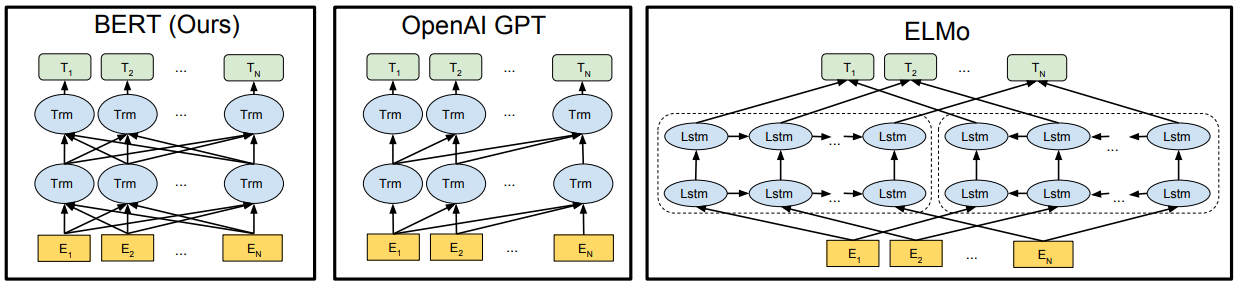
\includegraphics[width=150mm,scale=0.5]{obrazky-figures/Bert_porovnani.PNG}
    \caption{Rozdíly v~architekturách před trénovaných modelů. \textbf{BERT} používá oboustranný Transformer, \textbf{OpenAI GPT} používá pouze transformer \textit{zleva doprava}. \textbf{ELMo} používá zřetězení nezávisle trénovaných LSTM (Long short-term memory) \textit{zleva doprava} a \textit{zprava doleva} pro generování funkcí pro následné úkoly. Z~těchto tří architektur je pouze reprezentace BERT v~levém i pravém kontextu ve všech vrstvách. Architektury BERT a OpenAI GPT mají dolaďovací přístup, zatímco ELMo má přístup založený na funkcích. Převzato z~\cite{devlin2019bert}.}
    \label{fig:Bert_porovnani}
\end{figure}

\subsection*{Aspektově orientovaná analýza}

Další způsob určení polarity článku je možný na základě aspektů. Například věta \textit{Baterie vydrží dlouho, ale Hlasitost je nízká.} obsahuje dva aspekty, konkrétně \textit{Výdrž Baterie} a \textit{Hlasitost} produktu. Z~textu je třeba rozpoznat tyto aspekty, k~nim přiřadit slova je hodnotící a určit, jestli je aspekt ohodnocen pozitivně či negativně\cite{FITBT20346}.

Aspektově orientovaná analýza neprovede pouze rozlišení recenzí na pozitivní či negativní, ale navíc může sentiment roztřídit do kategorií, které jsou hodnoceny. To lze využít například u~zjištění, co se konkrétně zákazníkům nelíbí při hodnocení nějakého zařízení, je tak možné vyhledat rozdíl jestli se recenzentovi nelíbí hlučnost zařízení, ale líbí se mu třeba vzhled\cite{FITMT22451}.

\subsubsection*{Vyhledání aspektů}
Aspekty jdou získat pomocí modelu vytrénovaného strojovým učením. Tento způsob je vhodný pro vyhledávání informací stejného typu, například při zpracování recenzí hodnotící restauraci se budou často vyskytovat aspekty podobného typu jako například \textit{Jídlo} nebo třeba \textit{Personál}. Systém se naučí, jak tyto aspekty rozpoznat a poté může v~textu identifikovat, že se jedná o~hodnocení jídla, když recenzent napíše \textit{Nic mi nechutnalo}. Nevýhoda tohoto způsobu je, že potřebuje rozsáhlou datovou sadu, na které by se naučil aspekty rozpoznávat\cite{wang2015deep}.

Další způsob získání aspektu je pomocí gramatického zpracování textu, zejména určením stavby věty a závislostí jednotlivých slov ve větě. Tento způsob má výhodu v~tom, že není potřeba dopředu určit, jaké aspekty nás zajímají a systém sám vyhledá, jaké aspekty jsou ve větě obsaženy a jaké slova je hodnotí\cite{chockalingam2018}.

\subsubsection*{Větná stavba}
Pro určení aspektů pomocí větné stavby je třeba větu rozložit na jednotlivá slova, určit u~nich gramatické informace, jako jsou slovní druhy a závislosti ve větě. Pro tento úkol je v~práci využit český nástroj \textit{UDPipe}\footnote{\url{https://ufal.mff.cuni.cz/udpipe/2}}. Tento nástroj provede rozdělení věty na jednotlivá slova, přiřadí slovní druhy a určí závislosti slov ve větě. 

\chapter{Návrh řešení}
\label{navrh_reseni}
V~této kapitole jsou popsány jednotlivé části celé práce \ref{fig:navrh_systemu}, je zde uvedeno s~jakými daty která část pracuje a jejich bližším rozborem. Využití znalostní báze Wikidat v~práci, jakým způsobem je v~textu vyhledán relevantní text, tvorba datové sady, na které byla později práce testována. Postup, jakým způsobem jsou články hodnoceny, jestli se jedná o~recenzi či nikoli, rozpoznání názvu produktu. Jaké jsou v~práci speciální případy a co je u~nich jiného, popis konfiguračního souboru a postup, jakým byl určován sentiment článků.

\begin{figure}[h]
    \centering
    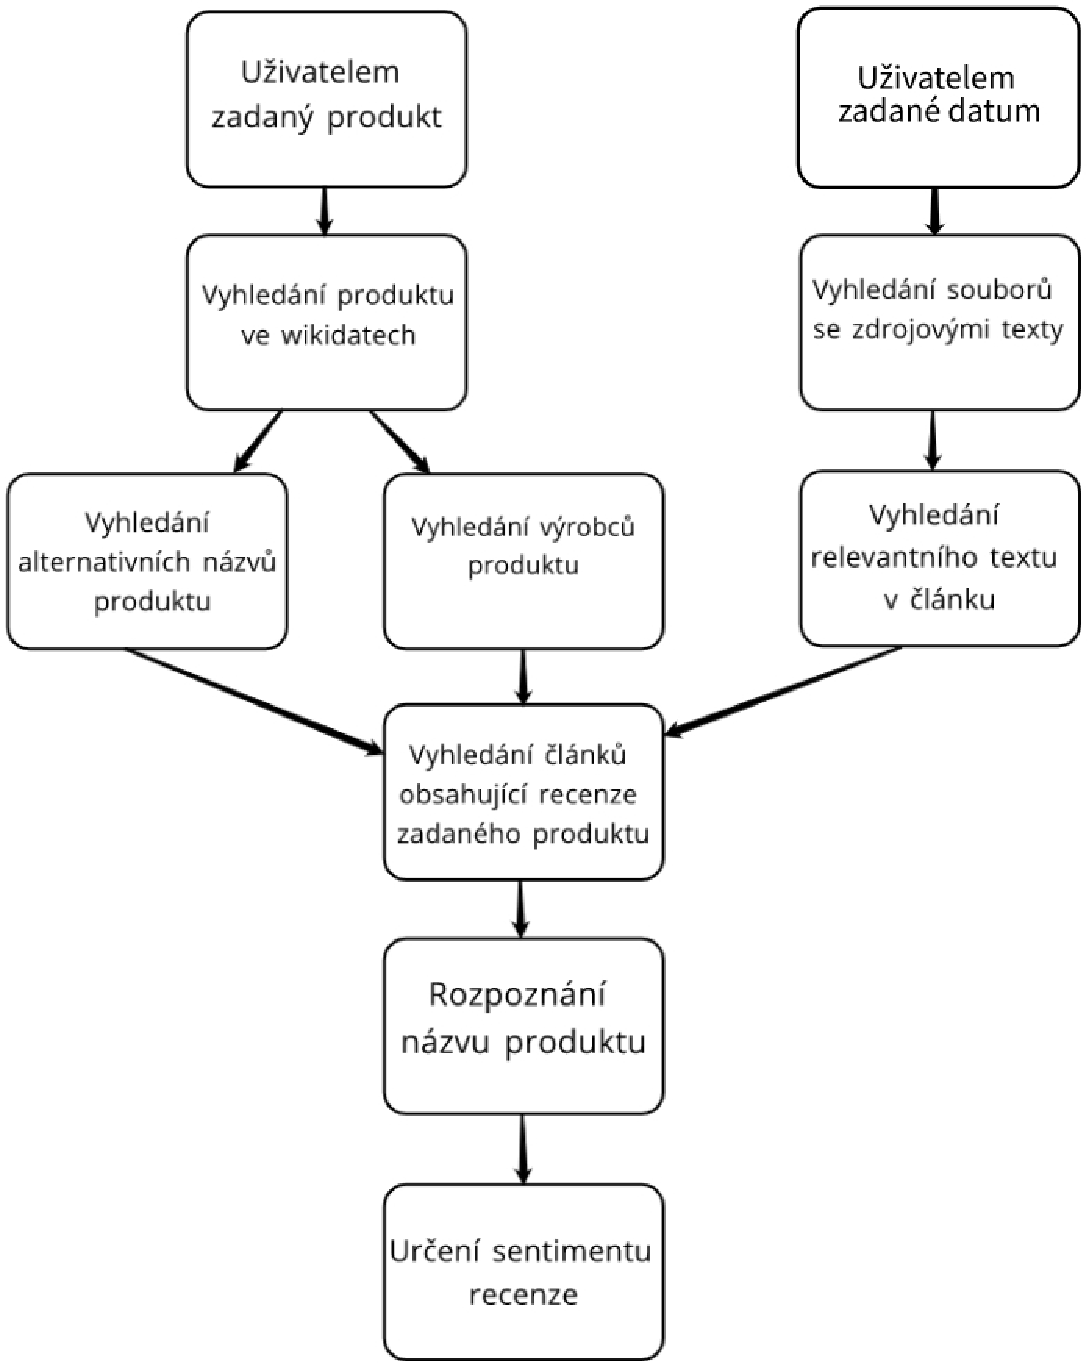
\includegraphics[scale=0.5]{obrazky-figures/navrh_systemu.pdf}
    \caption{Návrhu systému}
    \label{fig:navrh_systemu}
\end{figure}


\section{Dostupná data}
Práce používá data zpracované projektem \textit{FeedsCrawler}, které jsou uloženy na serveru \verb|minerva3| od výzkumné skupiny \verb|KNoT|. Přesná poloha dat je:
\begin{center}
\verb|/mnt/data-2/feeds_crawling/big_brother/workplace/4-tagged/cs_media/|
\end{center}
Skripty této práce budou hledat vstupní data v~tomto adresáři, je tedy třeba spustit práci z~tohoto serveru. Pro využití dat z~jiného adresáře je třeba upravit údaj v~konfiguračním souboru udávající polohu zdrojových dat.

\subsection*{Soubory vstupních dat}
Soubory jsou rozděleny po dnech, takže v~každém souboru jsou obsaženy všechny články vydané v~jeden den. Jednotlivé články souboru jsou rozděleny specifickými značkami. Obsah každého článku je dále pomocí dalších značek rozdělen na menší části, jako titulek, odstavce a jednotlivé nadpisy. V~prvním řádků každého článku je obsažena URL adresa článku, titulek a unikátní identifikátor. Podrobnější informace k~využitým značkám jsou uvedeny v~práci zabývající se tvorbou projektu \textit{FeedsCrawler}\cite{FITBT20846}.

\subsubsection*{Zpracovaný text}
Na následujícím obrázku je ukázán příklad jednoho řádku ze zpracovaných dokumentů. Jsou zde vyznačeny pouze informace důležité pro tuto práci, hodnoty jsou od sebe odděleny tabulátory.
Na obrázku \ref{fig:priklad_zpracovani_slova} je zobrazen příklad jednoho řádku ze vstupního souboru.

\smallskip

\begin{figure}[h]
    \centering
    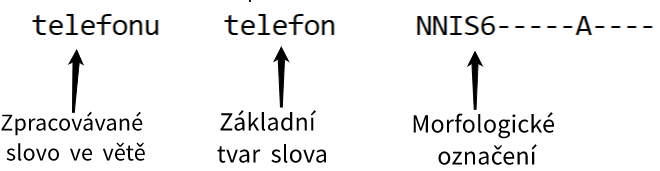
\includegraphics[scale=0.35]{obrazky-figures/priklad_zpracovani_slova.png}
    \caption{Ukázka jednoho řádku ze zpracovávaných dat}
    \label{fig:priklad_zpracovani_slova}
\end{figure}



\subsubsection*{Morfologické označení}
Tuto hodnotu přiřadí každému slovu nástroj \textit{MorphoDita}, který používá označování podle Českého Morfologického systému od Jana Hajiče \cite{hajic2004disambiguation}. Toto označení se skládá z~15ti pozic odpovídající části řeči, pohlaví, číslu, velikosti písmen atd\footnote{\url{https://ufal.mff.cuni.cz/pdt2.0/doc/manuals/en/m-layer/html/ch02.html}}. Pro tuto práci je nejdůležitější značka \verb|NN|, která indikuje, že se jedná o~podstatné jméno.

\subsection*{Výběr dnů ke zpracování}
Zpracování všech dnů od konce roku 2019, kdy projekt \textit{FeedsCrawler} začal stahovat články, by bylo časově náročné. Uživatel má možnost vybrat si dny, ve kterých se budou recenze vyhledávat. Výběr dnů ke zpracování je proveden při spuštění skriptu, uživatel zadá datum prvního a posledního dne a soubory nalezené mezi těmito daty jsou určeny ke zpracování. Pokud je počáteční i konečné datum stejné je zpracován pouze jeden den. 

\section{Použití wikidat}
Pro vyhledávání celé skupiny produktů je třeba najít alternativní názvy zadaného produktu, které se mohou v~hledaném článku vyskytnout, navíc jsou vyhledány firmy, které se daným produktem zabývají, protože jsou většinou také v~článcích zabývajících se hledaným produktem zmíněny.

K~vyhledávání těchto informací jsou použity Wikidata \ref{teorie:wikidata}, ve kterých práce vyhledává pomocí jazyku \textit{SPARQL}. 

\subsection*{Alternativní názvy produktu}
Podle zadaného produktu je ve Wikidatech podle názvu nalezena správná položka a jsou staženy její alternativní názvy v~Českém a Anglickém jazyce. Angličtina je stažena kvůli tomu, že se některé názvy moderních výrobků používají i v~česky psaném textu, například se často používá \textit{smartphone} na místo \textit{chytrý telefon}.

\subsection*{Výrobci produktu}
Z~názvu zadaného produktu je získán identifikátor výrobku. Poté jsou vyhledány všechny položky, které mají vlastnost \verb|product or material produced|(P1056) a jedna z~hodnot této vlastnosti je právě ID produktu.
U~položek, které odpovídají tomuto výroku, je vybráno jednoslovné označení z~oficiálního či alternativních názvů, pokud je dostupné. 

Jednoslovný název je lepší kvůli tomu, že v~článcích není většinou uveden celý oficiální název firmy jako třeba u~\textit{Volvo Cars} je většinou uváděno pouze \textit{Volvo}.

\section{Vyhledání relevantního textu}
Pro správné rozpoznání recenze je třeba vybrat pouze nadpisy a obsah článku\ref{fig:relevantni_text} kvůli tomu, že se v~textu často vyskytují odkazy na podobné články nebo je někde na stránce sekce \textit{Mohlo by vás zajímat}, která obsahuje mnoho dalších odkazů. Práce se tedy snaží vybírat pouze relevantní text. Odstranění reklam proběhne již při zpracování vstupních dat, dále je tedy potřeba odstranit menu webu, odkazy na podobné články a nepotřebné informace jako například jméno autora článku.

Relevantní text se nachází v~hlavičce článku, nadpisech, podnadpisech a samotných odstavcích. Vyhledání hlavičky a nadpisů není problém, protože jsou ve zpracovaných datech označeny specifickými značkami pro hlavičku, nadpisy a podnadpisy.

Pro vyhledání správných odstavců je použitý počet vět v~odstavci, ze kterých se text skládá. Věty v~odstavcích jsou oddělené značkami, není tedy problém zjistit jejich počet. Sekce se souvisejícími články někdy mají krátký popisek obsahu, většinou tyto krátké popisky mají jednu dlouhou či dvě kratší věty.

\begin{figure}[h]
    \centering
    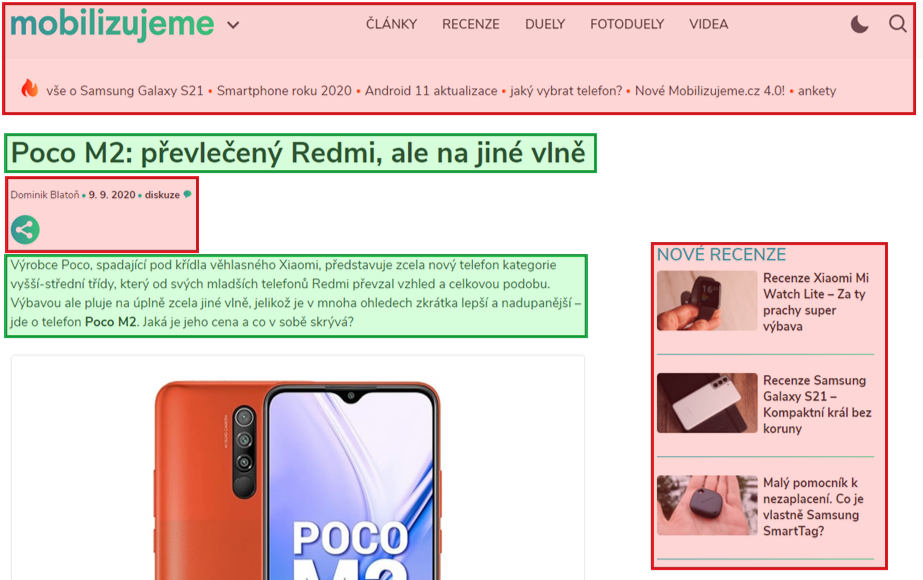
\includegraphics[scale=0.45]{obrazky-figures/ukazka_relevantniho_textu.png}
    \caption{Červeně je vyznačen nerelevantní text, který je v~článku přebytečný a je třeba ho odstranit, Zeleně je označen obsah článku důležitý pro tuto práci. Část obrázku převzata z~portálu \textit{mobilizujeme.cz}}
    \label{fig:relevantni_text}
\end{figure}


\section{Tvorba datasetu pro testování}

Pro tvorbu datasetu jsem manuálně prošel články ze dnů 10.09.2020 - 16.09.2020 ve kterých je dohromady stažených 18516 článků. Zaměřoval jsem se na vyhledávání článků obsahující recenze. Celkově jsem tak našel 80 článků, které jsem označil jako recenze. Vyhledané recenze jsem rozřadil do několika kategorií z~nich nejčastěji byly recenze telefonů a automobilů.

\subsection*{Kategorie a jejich počty}
Články rozřazené do kategorií a seřazené podle četnosti.
\begin{itemize}
    \item telefon: 25
    \item auto: 22 
    \item notebook: 7
    \item hardware: 6
    \item sluchátka: 5
    \item film: 5
    \item videohra: 4
    \item kniha:4  
\end{itemize}


\section{Rozpoznání recenze}
Při tvorbě datasetu jsem si všímal, podle čeho recenze identifikuji a zjistil, že ve většině případů jde rozpoznat, jestli se jedná o~recenzi nějakého produktu už z~adresy url článku. Článek s~adresou \textit{https://mobilenet.cz/clanky/recenze-motorola-moto-g-5g-plus-stredni-trida\--\-s\-e\--\-v\-sim-vsudy-41676}
lze označit za recenzi i bez otevření článku. Stejně jako u~url adresy {\textit{https://www.sport.cz/ostatni/basketbal/clanek/1663829-hrac-nba-mel-navstevu-na-pokoji\--\-z\-a\--trest\-\--byl-vyloucen.html\#rss}} jde vidět, že se o~recenzi jednat nebude. Pak jsou ještě články, u~kterých z~adresy nejde zjistit, o~čem se v~něm píše, protože v~URL neuvádějí část hlavičky, ale pouze unikátní identifikátor jako například \textit{http://www.halonoviny.cz/articles-/view/54232217}

I~přes to, že se dá recenze často identifikovat už z~url adresy, jsou zpracovávány celé články. Při zpracování skript prochází jednotlivé odstavce a v~případě, že je zpracovávaný text označen za relevantní, jsou zpracována jednotlivá slova odstavce. V~případě, že je slovo označeno jako podstatné jméno je porovnán jeho základní tvar se seznamem alternativních názvů produktů, výrobců a slov označující recenze. Pokud je základní tvar slova v~některém seznamu z~hledaných slov, je článku přičteno skóre které znázorňuje podobnost s~textem obsahující recenzi hledaného produktu.

\subsection*{Skóre článků}
Hodnota, která je článku přičtena při nalezení slova v~některém ze seznamů, záleží na několika aspektech, jako ve kterém ze seznamů bylo slovo nalezeno a taky, ve kterém odstavci. Pokud je například slovo \textit{Recenze} uvedeno v~hlavičce článku, je přičtena vyšší hodnota, než když je nalezeno jméno produktu v~obsahu článku. Přesné případy a hodnoty jsou uvedeny v~sekci \ref{zpracovani_odstavce}.

\subsection*{Výsledné články}
Po projití všech odstavců v~článku je podle skóre vyhodnoceno, jestli článek bude přidán do výsledků. Do výsledků je přidán článek, který v~textu či hlavičce obsahuje alespoň jedno slovo ze seznamu alternativních názvů, jedno slovo ze seznamu definující recenze a skóre vyšší či rovno hodnotě 30.

Když je článek označen jako recenze, proběhne rozpoznání názvu produktu. Po prohledání všech vstupních souborů jsou výsledné články seřazeny podle skóre a je u~nich vyhodnocen sentiment.

\subsection*{Rozpoznání názvu produktu}

Název je rozpoznán na základně jednoduchých gramatických pravidel. Vyhledávání názvu pomocí strojového učení by pro tuto práci vyžadovalo velkou datovou sadu, aby se model naučil rozpoznávat produkty všech typů.

Protože bývá název produktu, kterým se článek zabývá uveden v~hlavičce článku, použil jsem pro identifikaci názvu produktu jednoduchou extrakci slov z~titulku. Jsou vybrány slova začínající velkými písmeny a číslovky, navíc jsou odstraněny slova, podle kterých bylo určeno, že se jedná o~recenzi. Vybraná slova jsou poté porovnána s~url adresou a jako název označena pouze ty, která se vyskytují v~url adrese i titulku článku.

Název produktu je poté ověřen vyhledáním produktu na portálu \textit{heureka.cz} a porovnáním prvních výsledků vyhledávání.

\section{Speciální případy}
Pro některé typy produktu byly přidány speciální podmínky rozpoznání názvu. Tyto speciální případy jsou hlavně pro produkty, kde rozpoznání na základě velkých písmen není možné, jako například u~knih, filmů a počítačových her. Tyto případy mají předem určené weby, na kterých hledat jaký produkt. Tímto způsobem je tedy možné pro každý portál předem určit způsob vyhledání názvu, protože si weby drží stejný formát HTML pro určitý typ produktu, lze hledaný název vyhledat pomocí HTML kódu.

Speciální případy s~weby, na kterých se mají tyto produkty hledat a kódem pro každý web jsou uloženy v~konfiguračním souboru. Poté, co jsou vyhledány alternativní názvy hledaného produktu je prohledán tento soubor, jestli jeden z~alternativních názvů není speciálním případem, pokud ano je s~produktem zacházeno, jako se speciálním to znamená, že recenze budou vyhledávány pouze na portálech uvedených u~daného speciálního případu a pro hledání nazvu produktu bude využit předurčený kód pro každý z~webů. 

\section{Konfigurační soubor}

Tento malý textový soubor poskytuje hlavnímu skriptu informace důležité pro chod systému. Obsahuje cestu ke vstupním datům, se kterými skript pracuje a podmínky zpracování speciálních případů.

Konfigurační soubor je napsán formou slovníku jazyka \textit{Python}, je tedy potřeba dodržovat přesný formát zápisu.

Každý případ, který by měl mít speciální podmínky hledání názvu produktu, musí mít uvedené klíčové slovo určující, že se jedná o~speciální případ. Vypsané portály, na kterých se budou články vyhledávat a kód, pomocí kterého se v~článku najde název produktu. Rozložení tohoto souboru je vyobrazeno na obrázku \ref{fig:ukazka_konfigu}. 

\begin{figure}[h]
    \centering
    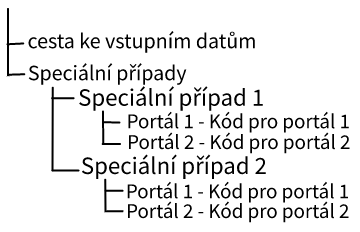
\includegraphics[scale=0.45]{obrazky-figures/ukazka_konfigu.png}
    \caption{Rozložení konfiguračního souboru}
    \label{fig:ukazka_konfigu}
\end{figure}


\subsection*{Zápis kódu}
Výsledek kódu pro hledání názvu je třeba zapsat do proměnné \verb|ArticleProduct| a celý kód vložit do trojitých uvozovek. Pro vyhledávání v~HTML lze použít proměnnou \verb|page_soup|, která obsahuje HTML stránky zpracované nástrojem \textit{BeautifulSoup}.

\section{Určení sentimentu}
U~článků je ohodnocen sentiment autora recenze, hlavně jestli recenzent hodnotí produkt pozitivně či negativně. Primárně je sentiment určován na základě aspektů. V~textu zpracovávaného článku jsou vyhledány aspekty produktu a jejich hodnocení, poté je určeno, jak jsou jednotlivé aspekty ohodnoceny. Pokud se v~textu nezdaří vyhledat žádné vhodné slova na základě kterých by šel aspekt ohodnotit, je provedena analýza sentimentu pomocí modelu BERT společně s~knihovnou \textit{Transformers} od společnosti \textit{Huggin Face}\footnote{\url{https://huggingface.co/}}.

\subsection*{Aspektová analýza}

Pro vyhledání aspektů jsem zvolil způsob určování na základě větné stavby. Vyhledávání na základě strojového učení není v~tomto případě vhodné, protože práce musí zpracovávat různé produkty a pro naučení modelu, který by spolehlivě vyhledával aspekty ve všech produktech, by bylo potřeba vytvořit velkou datovou sadu.

Sentiment je určován až poté, co je článek vyhodnocen jako recenze. Aby byly aspekty vyhledávány pouze v~relevantním textu, je obsah zpracovávané stránky stažen a zpracován nástrojem \textit{justext}, který vyhledá text vhodný ke zpracování. Tento text je poté zpracován knihovnou \textit{udpipe}. Tato knihovna obsah článku rozdělí na jednotlivé věty a určí větnou stavbu \ref{fig:zpracovani_vety}. Jednotlivá slova mají přiřazeny slovní druhy a vztahy mezi slovy. Ze slov je odstraněna interpunkce a slova, která nenesou žádné informace. Dále jsou na základě slovních druhů a vztahů mezi slovy jsou vyhledány aspekty a jejich hodnocení.

Sentiment slov hodnotící aspekty je určen pomocí lexikonů negativních a pozitivních slov. Po prohledání celého textu je porovnán počet pozitivně a negativně ohodnocených aspektů, na základě vyššího počtu je pro celý článek určen sentiment. 

\subsubsection{Využité lexikony}
Aspektová analýza využívá pro určení sentimentu tři lexikony, první dva se zabývají určením, jestli je vyhledaný aspekt ohodnocen pozitivně či negativně. Poslední lexikon obsahuje takzvané \textit{Stopslova}, což jsou slova, která ve větě neobsahují žádné informace a nejsou tak pro určení aspektu či hodnocení důležitá, typicky se jedná o~spojka či předložky, v~českém jazyce jsou to slova například \textit{aby}, \textit{ale}, \textit{být}.

Lexikon pro rozlišení negativních a pozitivních slov byl poskytnut společností \textit{Kaggle}\footnote{\url{https://www.kaggle.com/}}, která se zabývá tvorbou volně dostupných datových sad pro využití při strojovém učení.

Slovník obsahující stopslova byl poskytnut webem \textit{countwordsfree.com}\footnote{\url{https://countwordsfree.com/}}, který se zabývá počtem slov v~textech určitého jazyka a tvoří tak datové sady stopslov pro různé jazyky.

\begin{figure}[ht]
    \centering   
    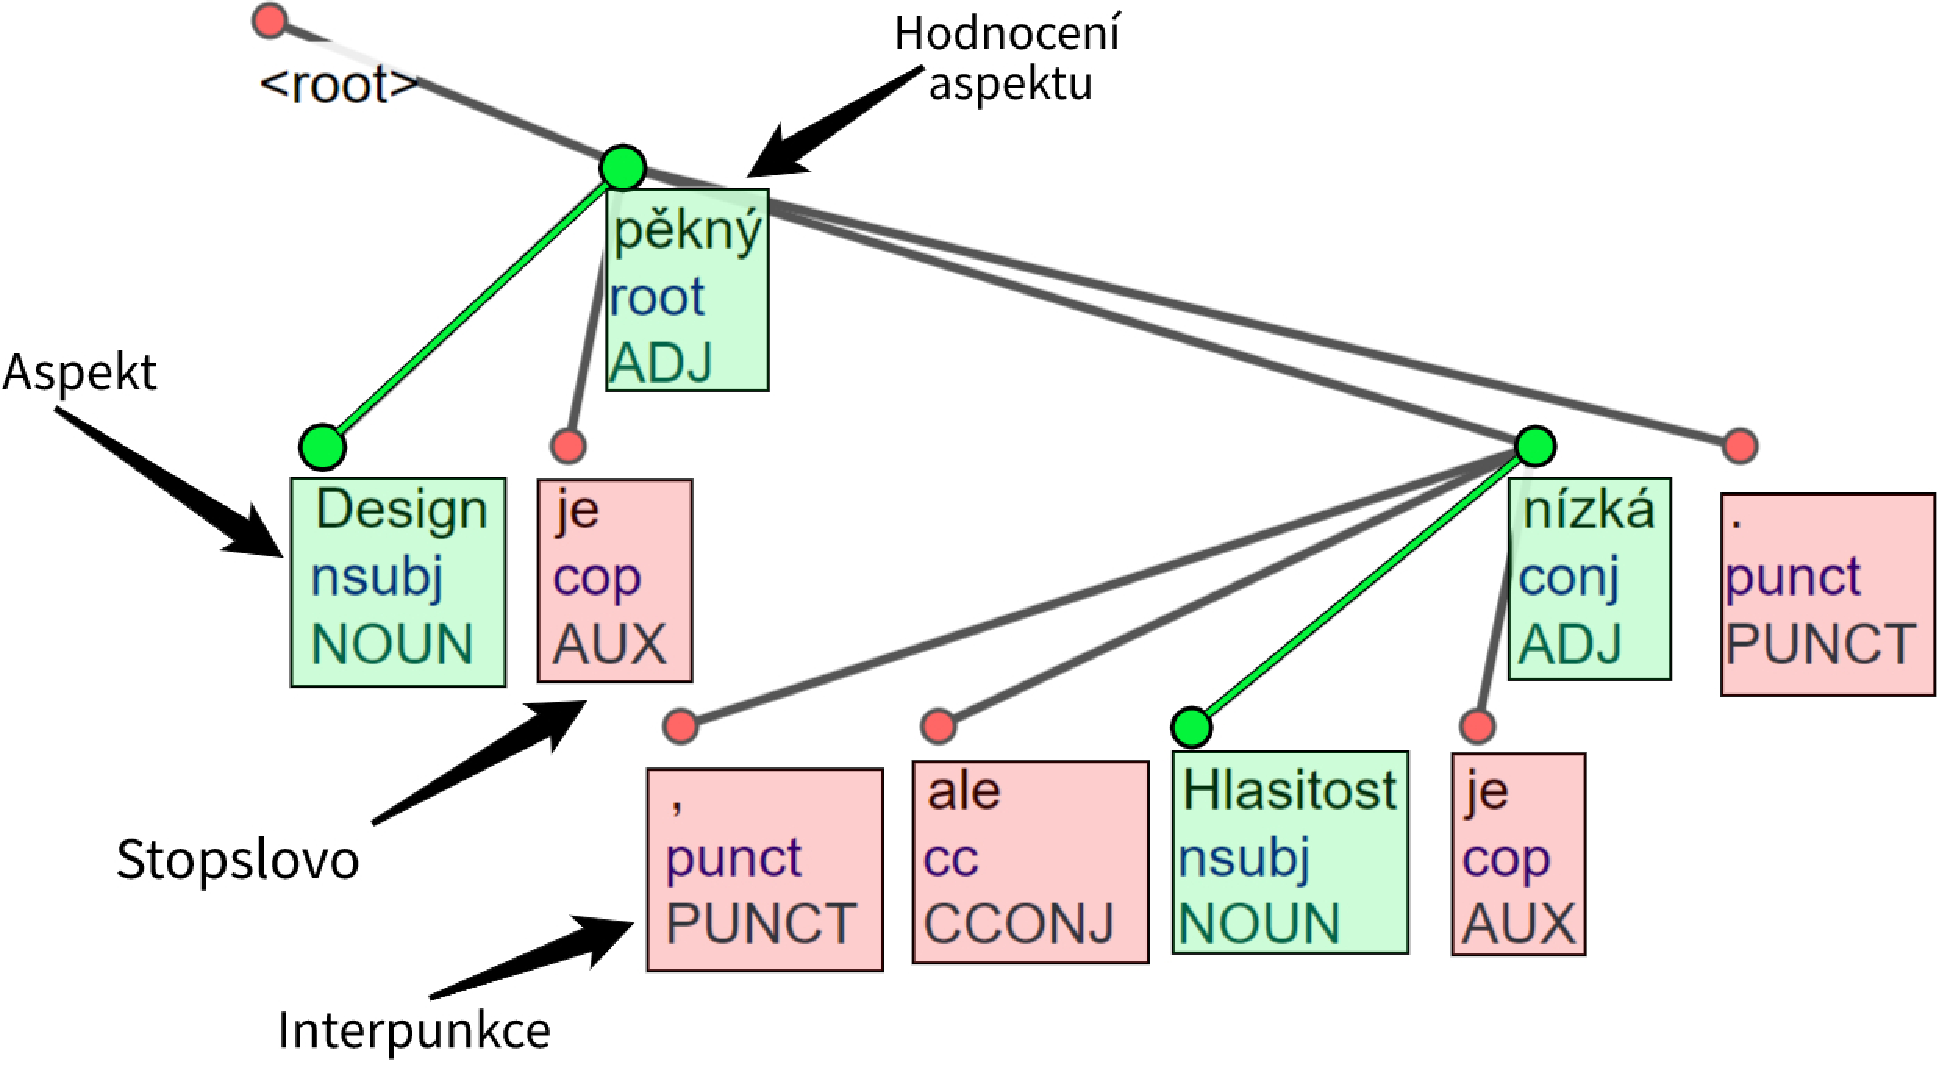
\includegraphics[scale=0.45]{obrazky-figures/zpracovani_vety.pdf}
    \caption{Ukázka zpracování věty nástrojem \textit{udpipe}. Zeleně jsou vyznačeny aspekty a jejich hodnocení. Červeně jsou označeny části věty odstraněné z~rozpoznání aspektů. Část obrázku převzata z~online ukázky nástroje \textit{udpipe}}
    \label{fig:zpracovani_vety}
\end{figure}


\subsection*{Určení sentimentu pomocí modelu BERT}

Pro určení sentimentu byl použit model BERT společně s~knihovnou \textit{Transformers} od společnosti \textit{Huggin Face}. Tento způsob jsem zvolil, protože má dostupný mnoho před-trénovaných modelů včetně několika modelů podporující český jazyk. 

\subsection*{Zpracování vstupního textu}
Modely určující sentiment pracují pouze s~čísly. Před tím, než bude u~článku určen sentiment. Je nejprve potřeba vstupní text zpracovat do číselné podoby, se kterou umí modely pracovat. Pro převod do číselné podoby lze využít modely společnosti \textit{Huggin Face}. Konkrétně jsem použil model \textit{DeepPavlov/bert-base-bg-cs-pl-ru-cased} určený pro zpracování slovanských jazyků, tento model byl trénován na článcích Wikipedie pro Bulharský, Polský, Český a Ruský jazyk a také na Ruských novinkových portálech.

S~využitím tohoto modelu je vstupní text převeden na seznam čísel, se kterým dále pracuje model vytrénovaný na určování sentimentu.

\subsection*{Ohodnocení sentimentu}
Sentiment je určen pomocí modelu natrénovaného na článcích, u~kterých bylo ručně určeno, jestli se jedná o~pozitivně či negativně hodnotící recenzi. Vyhodnocení sentimentu počítá i s~aspektem podnadpisů, kterým dává vyšší váhu na výsledek ohodnocení článku.

Skript obsahuje funkci, která ohodnotí článek ze zadané URL adresy pomocí vytrénovaného modelu,  nejprve je stažen obsah stránky, který je následně zpracován nástrojem \textit{justext}. Tento nástroj vyhledá relevantní text vhodný k~ohodnocení, odstraní související články a nepotřebné informace, takže ze stránky získáme pouze text vhodný k~ohodnocení a podnadpisy článku. Text je poté rozdělen podle odstavců a u~každého odstavce a podnadpisu je určen sentiment. Po ohodnocení všech vhodných textů je jejich výsledek zprůměrován a podle průměru je určeno, jestli se jedná o~pozitivní či negativní článek.

\subsection*{Trénování modelu}

Model byl trénován na článcích vyhledaných při tvorbě datasetu pro testování. U~těchto článků bylo poté manuálně určeno, jestli recenze obsahuje pozitivní či negativní hodnocení. Dále byl článek ručně rozdělen podle odstavců a u~každého odstavce určen sentiment na základě celého článku. Takže pokud recenze hodnotila produkt pozitivně, všechny odstavce v~textu byly označeny za pozitivní.

Model se zaměřuje na profesionálně napsané recenze, takže se dá předpokládat, že články nebudou obsahovat pravopisné chyby, se kterými by mohly být problémy při hodnocení recenzí psaných uživateli.

\chapter{Realizace}
\label{realizace}

Práce je psaná ve skriptovacím jazyce Python 3.6.9 a počítá s~tím, že je spuštěna na serveru minerva3 výzkumné skupiny KNOT. Skripty musí být spuštěny z~tohoto serveru, protože jsou zde dostupná zpracovaná data projektu \textit{FeedsCrawler}. Na serveru minerva3 lze skripty spustit z~domovském adresáře projektu \verb|/mnt/minerva1/nlp/projects/sentiment10|

V~této kapitole jsou podrobně popsány funkce jednotlivých skriptů, a jak fungují. Práce využívá následující skripty a soubory:

\begin{itemize}
    \item \verb|brandFinder.py| - ve wikidatech vyhledá alternativní názvy pro zadaný produkt a výrobce zadaného produktu.
    \item \verb|findReviewArticles.py| - hlavní skript, vyhledá články mezi dvěma daty obsahující recenze zadaného produktu.
    \item \verb|productFinder.py| - potvrzení, že zadaný produkt je platný.
    \item \verb|SentimentAnalyzerAspect.py| - analýza jestli je vyhledaná recenze pozitivní nebo negativní.
    \item \verb|udpipeParse.py| - vyhledání aspektů a jejich hodnocení pomocí větné stavby.
    \item \verb|morphoditaTagger.py| - doplnění textu o~slovní druhy a základní tvary slov pro přesnější vyhledávání recenzí.
    \item \verb|config.txt| - konfigurační soubor.
\end{itemize}

Při spuštění hlavního skriptu \verb|findReviewArticles.py| jsou nejprve vyhledány alternativní názvy zadaného produktu a firmy, které se výrobou daného produktu zabývají. Proběhne čtení konfiguračního souboru, vyhledání vstupních souborů mezi zadanými daty a paralelní vyhledání recenzí ve vstupních souborech. Jakmile jsou vyhledány recenze je u~nich určen sentiment a jsou vypsány na standardní výstup a seřazeny podle pravděpodobnosti, že se opravdu jedná o~článek zabývající se recenzí daného produktu. Články jsou seřazeny sestupně, takže na posledním řádku je článek nejvíce se podobající recenzi.

Průběh jednotlivých kroků, které skripty vykonávají, je podrobně popsán v~následujících sekcích.

V~průběhu skriptu je postup aktuálního zpracování ukazován na chybovém výstupu pomocí knihovny \textit{tqdm}. Výpis postupu \ref{fig:vypis_zpracovani} poskytuje informace o~procentuálním postupu práce s~grafickým znázorněním, počet již zpracovaných souborů, délka zpracování, předpokládaný čas do dokončení práce a průměrná délka zpracování jednoho souboru.
\begin{figure}[h]
    \centering
    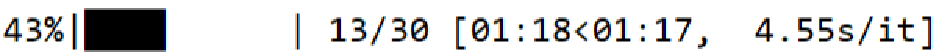
\includegraphics[scale=0.5]{obrazky-figures/vypis_zpracovani.pdf}
    \caption{Ukázka výpisu na chybovém výstupu v~průběhu zpracování.}
    \label{fig:vypis_zpracovani}
\end{figure}

\section{Použití wikidat}
Wikidata jsou využita pro vyhledávání alternativních názvů produktu a firem či výrobců, kteří se daným produktem zabývají. Pro vyhledávání je použit dotazovací jazyk \textit{SPARQL} a pro jeho používání v~jazyce Python práce používá modul \verb|SPARQLWrapper|, dále je pro vyhledávání využita API Wikidat. Výsledky hledání ve Wikidatech jsou vráceny ve formátu \verb|json|. Tato část práce probíhá ve skriptu \verb|brandFinder.py|.

\subsection*{Názvy produktu}
Vyhledání názvů probíhá ve funkci \verb|findProductNames(product)|, vstupní parametr je název produktu, pro který se mají vyhledat alternativní názvy. Zadaný řetězec je poté vyhledán ve Wikidatech voláním API wikidat na adrese \textit{https://www.wikidata.org/w/api.php} s~parametry:

\begin{lstlisting}[language=SPARQL]
    params = {
        'action': 'wbsearchentities',
        'format': 'json',
        'language': 'cs',
        'search': query
    }
\end{lstlisting}

poslední parametr \verb|search| má jako hodnotu proměnnou \verb|query|, která obsahuje řetězec \verb|product| vložený jako vstupní parametr funkce.

Tento příkaz ve Wikidatech vyhledá hledaný řetězec. Skript si dále uloží identifikátor první vyhledané položky do proměnné \verb|WikidataID|. 

Pomocí identifikátoru je vyhledána konkrétní položka a do seznamu \verb|result| vloženo označení položky v~českém a anglickém jazyce a také všechny alternativní názvy v~těchto jazycích. Nakonec je ještě tento seznam prohledán cyklem, který vyhledává slova obsahující diakritiku, pokud je takové slovo nalezeno, je do seznamu přidáno ještě jednou bez diakritiky.

Po dokončení těchto kroků funkce vrací seznam \verb|result| obsahující označení a alternativní názvy zadaného produktu v~českém a anglickém jazyce.

\subsection*{Názvy firem a výrobců}

Vyhledání názvů firem a výrobců je záležitost funkce \verb|findBrands(product)| tato funkce, stejně jako u~vyhledání alternativních názvů nejprve vyhledá položku zadanou vstupním parametrem ve Wikidatech pomocí API wikidat pro získání identifikátoru položky, který je opět uložen do proměnné \verb|WikidataID|.

Dále jsou pomocí následujícího dotazu v~jazyce SPARQL vyhledány položky zabývající se výrobou hledaného produktu. Dotazy SPARQL lze otestovat online\footnote{\url{https://query.wikidata.org/}}.

\begin{minipage}{\linewidth}
\begin{lstlisting}[language=SPARQL]
SELECT ?item ?itemLabel(GROUP_CONCAT(DISTINCT(?altLabel);separator=",")
AS ?altLabel_list)
WHERE {
  ?item wdt:P1056 wd:"""+WikidataID+""" .
  OPTIONAL {?item skos:altLabel ?altLabel .FILTER(lang(?altLabel)="en")}
  SERVICE wikibase:label { bd:serviceParam wikibase:language "en" .}
}
GROUP BY ?item ?itemLabel
\end{lstlisting}
\end{minipage}

Tento dotaz vyhledá všechny položky, které mají vlastnost \textit{product or material produced} (P1056) a v~této vlastnosti uvedenou položku s~identifikátorem uvedeným v~proměnné \verb|WikidataID|. Z~položek, které odpovídají tomuto výrazu, je uloženo označení položky a její alternativní názvy. Výsledek je ve formátu \verb|json|.

\begin{table}[h]
    \centering
    \begin{tabular}{||c|c|c||} 
        \hline
        item & itemLabel & altLabel\_list\\ [0.5ex] 
        \hline\hline
        Q6686 & Renault & Groupe Renault, Renault S.A., Renault SA \\ 
        \hline
        Q6742 & Peugeot & 	Peugeot Automobiles \\
        \hline
        Q6746 & Citroën & Automobiles Citroën S.A., Citroen \\
        \hline
        Q29637 & Škoda Auto & Skoda, Automobilový koncern ŠKODA a.s., ŠKODA \\
        \hline
    \end{tabular}
    \caption{Část výsledku vyhledání výrobců pro položku "automobil"(Q1420)}
    \label{tab:vyhledani_vyrobcu}
\end{table}

 V~případě, že je označení výrobce víceslovné, jsou prohledány alternativní názvy, jestli se v~nich nenachází název jednoslovný, který je pro vyhledávání v~článcích lepší, protože jsou články rozděleny na jednotlivá slova a víceslovný název by tak nebyl detekován.
 
 Vyhledané názvy jsou vloženy do seznamu \verb|brandList|, který je po prohledání všech výrobců vrácen jako výsledek funkce.

\section{Výběr souborů ke zpracování}

Soubory ke zpracování jsou vybrány na základě uživatelem zadaných vstupních argumentů a konfiguračního souboru. Nejprve je vytvořen seznam všech souborů adresáře zadaného parametrem \verb|dataSource| v~konfiguračním souboru. Poté jsou data zadané uživatelem zpracovány knihovnou \verb|dateTime| a v~seznamu všech souborů vyhledány dny nacházející se v~intervalu dvou dat, které zadal uživatel.

\subsection*{Formát dat}

Datum je třeba zadat ve specifickém formátu, aby s~ním knihovna \verb|dateTime| byla schopna dále pracovat. Vstupní soubory jsou zadané ve formátu \textbf{[YYYY]-[mm]-[dd]}, zvolil jsem tedy tento formát i pro argumenty při spuštění skriptu. Datum je třeba zadat včetně pomlček mezi hodnotami, příklad správně zadaného data: \verb|2021-3-20| = 20. března 2021

\section{Určovaní recenzí}
Vyhledání recenzí probíhá ve funkci \verb|readReviews(link)|, v~této funkci je vytvořena proměnná \verb|reviewWordsListPart|, která obsahuje řetězce, podle kterých se určuje, jestli článek obsahuje recenzi nebo ne. Řetězce použité pro identifikaci recenzí:
\begin{center}
    \verb|reviewWordsListPart = ['recenze','hodnoceni','test']|
\end{center}Pro vyhledání vhodných slov pro rozlišení recenze od ostatních článků jsem prošel recenze z~datové sady a všechny články rozdělil na slova a vytvořil slovník jejich četnosti. Abych se vyhnul slovům, která se vyskytují v~článcích, které recenze neobsahují jsem prošel i několik článků bez recenzí a sledoval, která slova se často vyskytují ve všech článcích.

Tato funkce vyžaduje parametr \verb|link|, který obsahuje odkaz na zpracovávaný datový soubor, ve kterém se mají recenze vyhledávat. Jednotlivé články tohoto souboru jsou rozděleny podle řetězce \textbf{<doc}, který se nachází vždycky na začátku nového článku. 

Cyklus postupně prochází všechny články ve zpracovávaném souboru, z~prvního řádku článku určí URL adresu zpracovávané stránky. Z~URL adresy si skript zjistí několik informací, proběhne kontrola, jestli se jedná o~českou webovou stránku s~doménou \textit{.cz}, protože zdrojové soubory obsahují i stránky slovenské se kterými práce nepracuje. Dále je z~URL zjištěno, jestli se nejedná pouze o~odkaz na nový komentář, toto je zjištěno z~konce url adresy, která v~případě, že se jedná o~komentář, končí řetězcem a identifikátorem komentáře, například: \textit{\#comment-360411}, práce s~odkazy na komentáře nepracuje, aby nedošlo k~duplicitnímu zpracování stejného článku. Na konci zpracování prvního řádku proběhne ještě kontrola, jestli se nejedná o~vyhledávání speciálního produktu, a pokud ano tak, jestli je URL adresa v~seznamu adres pro právě zpracovávaný produkt.

Po přečtení prvního řádku proběhne zpracování zbytku článku. Skript prochází soubor řádek po řádku a kontroluje jednotlivé slova a značky. V~průběhu si skript ukládá informace o~aktuálně zpracovávaném odstavci a až narazí na značku \verb|<\p>|, která udává konec odstavce je celý odstavec zpracován podle značek nalezených při jeho zpracování. Značky, které skript vyhledává při zpracování odstavce:
\begin{itemize}
    \item \verb|<head>| značka indikující, že se jedná o~hlavičku dokumentu, nastaví proměnnou\\* \verb|ArticleHeadFlag| na hodnotu \verb|True|.
    \item \verb|<s>| značení konce věty. Když skript narazí na tuto značku, zvedne počítadlo počtu vět \verb|ParagraphTagsS| ve zpracovávaném odstavci.
    \item \verb|<h>|: značka indikující, že se jedná o~nadpis či podnadpis v~textu, nastaví hodnotu proměnné \verb|ParHeading| na \verb|True|.
    \item \verb|<\p>|: značka konce odstavce. Jakmile skript narazí na tuto značku začne jeho zpracování.  
\end{itemize}

Než je odstavec zpracován je u~něj provedena kontrola, jestli se jedná o~relevantní text, toto je provedeno následující podmínkou.
\begin{center}
    \verb|if(ParagraphTagsS>2 or ArticleHeadFlag or ParHeading):|
\end{center}

Odstavec je tedy zpracován, pokud obsahuje více než 2 věty nebo se jedná o~hlavičku článku či podnadpis. V~případě, že je text vyhodnocen jako relevantní jsou v~něm vyhledána klíčová slova a podle toho ohodnocen článek.

\subsection*{Zpracování odstavce}
\label{zpracovani_odstavce}
Poté, co je odstavec vyhodnocen jako vhodný ke zpracování jsou nastaveny váhy výskytů slov určitého typu. Například pokud je v~textu slovo ze seznamu názvů produktu, je přičtena výsledku článku hodnota určena váhou slov z~právě tohoto seznamu.  

Tato váha je určená podle toho, jestli se jedná o~titulek článku či nikoli. V~případě, že se jedná o~titulek jsou nastaveny tyto hodnoty na:
\begin{itemize}
    \item \verb|BrandWeight|=10 - hodnota určující váhu slov ze seznamu firem či výrobců produktu.
    \item \verb|ProductWeight|=20 - hodnotu určující váhu slov ze seznamu názvů.
    \item \verb|ReviewWeight|=30 - hodnota určující váhu slov ze seznamu indikující recenze.
\end{itemize}
V~opačném případné jsou tyto hodnoty nastaveny na
\begin{itemize}
    \item \verb|BrandWeight|=0.5 
    \item \verb|ProductWeight|=10
    \item \verb|ReviewWeight|=0 
\end{itemize}
Hodnota \verb|ReviewWeight| je nastavená na 0 při vyhledávání v~textu článku, protože často bývají v~článku odkazy na recenze podobných produktů, tudíž by článek mohl být vyhodnocen jako recenze pouze na základě toho, že se někde v~článku takový odkaz nachází. Hodnota \verb|BrandWeight| je nastavena na 0.5, aby nebyly detekovány články, ve kterých je sice zmíněn výrobce hledaného produktu, ale článek se tímto produktem nezabývá, většina hledání tedy proběhne již v~hlavičce článku a zbytek textu slouží pouze ke zjištění, jestli se jedná o~článek zabývající se hledaným produktem. 

Každý zpracovávaný řádek je rozdělen podle znaku \verb|\t|, čímž se z~řádku vytvoří seznam informací o~slově, který je vložen do proměnné \verb|lineList|. U~každého slova je provedena kontrola, jestli se jedná o~podstatné jméno, toto je zjištěno z~hodnoty uložené na pozici \verb|lineList[2]|, která obsahuje morfologické informace o~zpracovávaném slově. Tyto informace jsou prezentovány formou řetězce, o~podstatné jméno se jedná, pokud řetězec obsahuje podřetězec \textit{NN}. 
V~případě, že se jedná o~podstatné jméno, je základní tvar zpracovávaného slova, který je uložen na pozici \verb|lineList[2]| porovnán se seznamy obsahující hledaná slova. Pro přesnější porovnání je základní tvar slova převeden na malá písmena při vyhledávání názvu produktu a recenze.

\subsection*{Označení recenze}
Článek je označen za recenzi, pokud obsahuje alespoň jeden výskyt názvu produktu, jedno slovo ze seznamu recenzí a jeho výsledná hodnota je vyšší či rovna hodnotě 30. Tuto hodnotu jsem zvolil tak, aby u~každého produktu, který bude uživatel hledat, byl vyhledán alespoň nějaký článek. Maximální výsledná hodnota článků se výrazně liší podle produkt, který uživatel vyhledává. 

Poté, co je článek vyhodnocen proběhne určení názvu produktu a výsledek je přidán do slovníku \verb|resultDict|. Článek je vložen do slovníku pod klíčem jeho URL adresy a jako hodnoty jsou do slovníku vloženy:
\begin{itemize}
    \item \verb|WordResult| - Výsledné skóre článku 
    \item \verb|IsBrand| - počet výskytů názvu výrobce v~textu článku
    \item \verb|IsProduct| - počet výskytů názvu produktu v~textu článku 
    \item \verb|IsReview| - počet výskytů slov recenzí v~textu článku
    \item \verb|ArticleProduct| - název produktu kterým se článek zabývá
    \item \verb|urlName| - název portálu na kterém se článek nachází
\end{itemize}

Poté, co jsou zpracovány všechny články v~souboru vrátí funkce slovník \verb|resultDict|.

\section{Určování názvu produktu}

Určování názvu produktu probíhá jako součást funkce pro vyhledávání recenzí, název je určen až poté, co je článek označen za recenzi. Pokud se nejedná o~speciální produkt, je název článku určen na základě velkých písmen v~titulku článku a url adresy.

Skript rozdělí titulek článku na slova podle bílých znaků a vyhledá slova začínající velkým písmenem a číslovky, tyto slova a číslovky jsou poté porovnány s~URL adresou stránky. Pokud se vybraná slova v~této adrese nachází, jsou vloženy do proměnné \verb|ArticleProduct| reprezentující název produktu.

Po vyhledání názvu skript \verb|productFinder| provede ověření, jestli se jedná o~platný název produktu. Ověření probíhá ve funkci \verb|WebScrape_product(product)|. Vstupní parametr \textit{product}, který obsahuje řetězec s~vyhledaným názvem produktu je převeden do formátu vhodného pro vyhledávání převedením mezer na znak \textit{+}, poté proběhne hledání na webu \textit{heureka.cz}. Toto hledání je provedeno pomocí webscrapingu url adresy vytvořené spojením \textit{https://www.heureka.cz/?h\%5Bfraze\%5D=} a vyhledávaného řetězce. Poté, co je stažen HTML kód z~portálu \textit{heureka.cz} jsou prohledány titulky položek. Většinou pokud je zadán neplatný produkt tak vyhledávání nenajde žádnou položku na základě zadaného řetězce a produkt je tudíž označen za neplatný. V~případě, že hledání vrátí několik položek jsou porovnány titulky prvních dvou položek s~vyhledávaným řetězcem a na základě podobnosti je produkt vyhodnocen jako platný či neplatný. Porovnání řetězců probíhá pomocí třídy \textit{SequenceMatcher} z~Pythonovského modulu \textit{difflib}. Tato třída porovnává řetězce podle nejdelší souvislé shodné posloupnosti a poté pomocí metody \textit{ratio()} vrací hodnotu v~intervalu 0.0-1.0 kde vyšší číslo reprezentuje vyšší podobnost. Název je označen jako platný, pokud dosahuje podobnosti alespoň 0.3.

\subsection*{Speciální produkty}
Pro produkty, jejichž název nejde určit na základě velkých písmen, je třeba použít jiný způsob určení názvu. Název těchto produktů je vyhledán pomocí webscrapingu zpracovávaného článku. Protože je každý portál jiný a používá vlastní způsob zápisu HTML nelze vytvořit skript, který by vyhledal název na všech webech, je proto, tedy potřeba používat specifický kód pro každý portál. To znamená, že tyto produkty budou vyhledávány pouze na portálech, které mají určený kód specifikován. Speciální produkty, weby a kód pro určení názvu produktu jsou definovány v~konfiguračním souboru.

U~speciálních produktů je nejprve stažen obsah ve formě HTML a poté pomocí knihovny \verb|BeautifulSoup| je obsah zpracován a vložen do proměnné \verb|page_soup|. V~konfiguračním souboru je podle URL aktuálně zpracovávaného článku vyhledán kód, který z~proměnné \verb|page_soup| vyhledá název produktu a vloží jej do proměnné \verb|ArticleProduct|, se kterou skript dále pracuje stejně jako u~ostatních produktů.

\section{Paralelní zpracování}

Paralelní zpracování umožňuje spustit skript jako více procesů. Paralelizace je v~této práci využita pro zpracování několika souborů najednou funkcí \verb|readReviews(link)|. Soubory určené ke zpracování jsou uloženy v~seznamu \verb|CorrectDateFilesList|, ze kterého jednotlivé procesy vybírají soubory které ještě nebyly zpracovány, dokud není zpracován celý seznam. Po dokončení práce na souboru jsou výstupní hodnoty funkce \verb|readReviews(link)| přidány do seznamu \verb|resList|. Poté, co jsou zpracovány všechny soubory jsou položky seznamu \verb|resList| převedeny na slovník \verb|resultDict| pro další zpracování.

\subsection*{Počet procesů}
Počet, kolik procesů se má spustit najednou je specifikován jako vstupní argument při spuštění skriptu. Paralelní zpracování výrazně sníží délku zpracování všech souborů, ale je taky náročnější na paměť počítače, na osobním počítači který má 16 GB paměti, jsem mohl práci spustit maximálně na dvou procesech. 

\subsection*{Způsob paralelního zpracování}
Paralelní spuštění je implementováno tak, že je zpracováváno více souborů najednou, to se při testování ukázalo jako nejvlivnější na zrychlení zpracování. Tento způsob implementace při spuštění práce na zpracování pouze jednoho souboru nemá žádný vliv na délku zpracování.

Testoval jsem i zpracování jednoho souboru více procesy, ale to na snížení délky zpracování nemělo moc vliv.

\section{Určování sentimentu}

Určením sentimentu se zabývá skript \verb|SentimentAnalyzerAspect.py|, který je volán z~hlavního skriptu funkcí \verb|Sentiment_from_url(url)|.Tato funkce vrátí řetězec \textit{pos},\textit{neg} či \textit{??} na základě ohodnocení sentimentu textu článku. Nejprve se skript pokusí vyhodnotit článek na základě aspektové analýzy, v~případě že se nepovede pomocí tohoto způsobu určit hodnocení článku, je využita analýza sentimentu pomocí strojového učení.

\subsection*{Aspektová analýza}

Nejprve je stažen obsah článku z~URL adresy zadané jako vstupní parametr při spuštění funkce, obsah toho článku je poté zpracován nástrojem \textit{justext} pro vyhledání relevantního textu. Text vybraný tímto nástrojem je prohledáván po odstavcích a každý odstavec je zpracován skriptem \verb|udpipeParse.py|, který v~zadaném textu vyhledá aspekty a jejich hodnocení. Aspekty ze zpracovávaného odstavce jsou poté ohodnoceny na základě lexikonů pozitivních či negativních slov. Po porovnání počtu pozitivně a negativně hodnocených aspektů je článku přiřazen sentiment podle vyšší hodnoty, pokud se v~článku nepodaří určit sentiment na základě aspektů je volána funkce \verb|Sentiment_from_Articletext(ArticleText)|, která z~již staženého článku provede analýzu sentimentu pomocí strojového učení. 

\subsection*{Vyhledání aspektů a jejich hodnocení}

Tato část práce probíhá ve skriptu \verb|udpipeParse.py|, k tomuto skriptu je přistoupeno pomocí funkce {\verb|AspectAnalyse(txt)|}. Tato funkce vyhledá ve vstupním textu aspekty a jaká slova je hodnotí, jako vstupní parametr je očekávána věta či odstavec textu. Pro zpracování textu jsem využil nástroj \textit{udpipe} v~kombinaci s~modelem \verb|UD Czech PDT|. Nejprve je zadaný odstavec zpracován tímto nástrojem, který text rozloží na jednotlivé věty, určí základní tvary slov, jejich slovní druhy slov a jakou závislost na sobě ve větě mají\cite{chockalingam2018}. Tvorba tohoto skriptu byla inspirována článkem od Rohana Goela\cite{goel_2020}. 

Vstupní text je dále zpracováván po jednotlivých větách, do skriptu je vložen ze souboru \verb|stop_words_czech.txt| lexikon stopslov, při zpracování věty jsou v~základních tvarech slov vyhledávány stopslova a ta jsou z~věty odstraněna. Je tak vytvořena nová věta, která stopslova neobsahuje. Nová věta je opět zpracována nástrojem \textit{udpipe}, aby se vytvořili nové větné závislosti.

Na základě závislostí jsou vytvořeny dvojice slov, které na sobě závisí a jejich vztah je popsán pojmem definovaným ve využitém modelu. 

Ve zpracovávané větě jsou vyhledány slova označené jako podstatné či přídavné jména, na základě těchto slov je vytvořen seznam vlastností zpracovávané věty a průběžně je tvořen seznam vlastností celého odstavce. 

Poté je seznam vlastností porovnán se seznamem dvojic, jsou vyhledávány položky, které se nacházejí v~seznamu dvojic a zároveň v~seznamu vlastností, pokud je taková položka nalezena, je nahlédnuto na vztah dvojic, pokud je vztah dvou slov obsažen v~následujícím seznamu, obsahuje dvojice hodnocení některé z~vlastností.

\begin{lstlisting}[basicstyle=\small]
["nsubj", "acl:relcl", "obj", "advmod", "amod", "neg", "xcomp", "compound", "orphan", "acl", "conj",
 "appos"]
\end{lstlisting}

Tento seznam vztahů byl vytvořen podle článku Subhabrata Mukherjee a Pushpaka Bhattacharyya zaměřeného na aspektovou analýzu recenzí produktů\cite{mukherjee2012feture}, popis jednotlivých zkratek je v~dokumentaci použitého modelu\footnote{\url{https://universaldependencies.org/treebanks/cs\_pdt/index.html\#ud-czech-pdt}}.

Po prohledání všech vět ve zpracovávaném odstavci jsou vyhledány ve vlastnostech podstatná jména a ty označeny jako aspekty, na výstup funkce je poté vložen seznam Aspektů a ke každému aspektu přidán seznam slov, které tento aspekt hodnotí.

\subsection*{Ohodnocení na základě aspektů}
Výsledek hodnocení článku je určen proměnnou \verb|rating|. Aspekty a jejich hodnocení jsou vyhledávány zvlášť v~každém odstavci zpracovávaného článku, po vyhledání aspektů je nahlédnuto na všechna slova hodnotící tyto aspekty. Pokud je hodnotící slovo nalezeno v~lexikonu pozitivních slov, je inkrementována hodnota proměnné \verb|rating|, pokud je toto slovo nalezeno v~negativním lexikonu, je tato hodnota dekrementována. Po prohledání všech odstavců je pomocí proměnné \verb|rating| určen sentiment článku, pokud je její hodnota pozitivní je článku přiřazen pozitivní sentiment, v~opačném případě je přiřazen negativní sentiment, pokud je hodnota této proměnné rovna 0, je tento článek zpracován pomocí strojového učení.

\subsection*{Analýza sentimentu pomocí strojového učení}

Pro hodnocení sentimentu skript používá knihovny \textbf{PyTorch}, \textbf{TensorFlow 2.0} a \textbf{Transformers} pro vytvoření a použití modelu pro vyhodnocení sentimentu pomocí strojového učení.

Tento skript byl vytvořen podle článku od \textit{Venelina Valkova} zaměřující se na analýzu sentimentu recenzí aplikací na webu \textit{play.google.com}\footnote{\url{https://play.google.com/store}}\cite{valkov_2020}.

Nejlepší před trénovaný model, který jsem pro zpracování českého textu našel, byl
\begin{center}
 \textit{DeepPavlov/bert-base-bg-cs-pl-ru-cased}   
\end{center}
Tento model má problémy s~diakritikou, ale po odstranění diakritiky funguje docela dobře.

Na následujícím příkladu lze vidět průběh převedení české věty \textit{Auto je podle nás v~redakci velice povedené vozidlo} do tvaru vhodného pro určení sentimentu pomocí před trénovaného modelu.
\begin{lstlisting}[basicstyle=\small]
 Sentence: Auto je podle nas v~redakci velice povedene vozidlo.
   Tokens: ['Auto', 'je', 'podle', 'nas', 'v', 'redakci', 'velice', 'povede', '##ne', 'vozidlo','.']
Token IDs: [23265, 2053, 3874, 12947, 190, 88651, 16210, 101961, 2136, 60058, 119]
\end{lstlisting}

Některé slova byly rozděleny na dva tokeny, druhý token začíná značkou \verb|##| která naznačuje, že je součásti tokenu předchozího. Rozdělení nastane v~případě, že model, který větu zpracovává určité slovo nerozpozná a rozdělí ho na slova, které poznává.

Funkce \verb|Sentiment_from_url(url)| očekává jako vstupní parametr url adresu článku, u~kterého má být ohodnocen sentiment. Nejprve je stažen HTML kód zadané stránky, který je následně zpracován nástrojem \textit{justext} s~parametrem pro vyhledávání českého textu. A~text je poté postupně po odstavcích třídou \verb|SentimentClassifier| zpracováván a každý odstavec či podnadpis je pomocí vytrénovaného modelu ohodnocen. Výsledky ohodnocení se sčítají, poté jsou zprůměrovány a na základě průměru je vyhodnocen sentiment článku. Návratové řetězce funkce:
\begin{itemize}
    \item 'pos' - Sentiment článku byl vyhodnocen jako pozitivní 
    \item 'neg' - Sentiment článku byl vyhodnocen jako negativní
    \item '??'  - Sentiment článku se nepodařilo určit, tato situace nastane většinou v~případě že se obsah stránky nepodaří stáhnout nebo nástroj \textit{justext} nenajde na stránce žádný text vhodný ke zpracování.
\end{itemize}

\subsection*{Trénování modelu}
Trénování modelu probíhalo ve skriptu \verb|training.py|. Tento skript obsahuje několik tříd a funkcí popsaných níže. 

\subsubsection*{Tvorba Datasetu}
Nejprve jsem vytvořil dataset pro trénování. Dataset se skládá z~článků označených jako pozitivní či negativní recenze, tyto články jsou poté rozděleny na odstavce a z~nich vytvořen soubor \verb|trainingReviews.csv|, který je využit pro trénování modelu. Tento soubor obsahuje na každém řádku dvě hodnoty, text a sentiment a při jeho tvorbě je z~článků odstraněna diakritika.

Dataset se skládá celkem z~172 odstavců s~přiřazeným sentimentem, z~toho je 99 označeno jako pozitivní a 73 jako negativní. Pro trénování jsou tyto odstavce rozřazeny do tří kategorií:

\begin{itemize}
    \item Trénovací data - Data, na kterých se model učí.
    \item Validační data - Data použitá k~ověření přesnosti modelu při jeho učení.
    \item Testovací data - Data použitá pro otestování modelu po dokončení učení.
\end{itemize}

Dataset byl rozdělen na 155 testovacích odstavců, 8 validačních a 9 testovacích.

\subsubsection*{Průběh trénování}
Model Bert vyžaduje, aby počet tokenů ve všech zpracovávaných textech byl stejný, je proto zvolena konstanta \verb|MAX_LEN|, která udává počet, na který se bude počet tokenů zarovnávat, pokud je text delší, k~vyhodnocení sentimentu je použito pouze prvních X tokenů kde X je hodnota \verb|MAX_LEN| a zbytek textu odstřižen, v~opačném případě kde je počet tokenů nižší než maximum je zpracovávaný text doplněn prázdnými tokeny s~hodnotou 0, aby byla splněna požadovaná délka. Po projití odstavců v~datasetu jsem zvolil hodnotu \verb|MAX_LEN|=200.

Model BERT používá několik speciálních tokenů, které je potřeba do textu doplnit, aby šlo text zpracovat, dále je potřeba text upravit, aby šel zpracovat pomocí knihovny \verb|PyTorch|. O~přidávání těchto tokenů a zpracování textu se stará tokenizer, který metodou \verb|encode_plus| tokeny automaticky doplní a text zpracuje. Tato metoda je pro správné zakódování spouštěna s~následujícími parametry:

\begin{lstlisting}[basicstyle=\small]
encoding = tokenizer.encode_plus(
  review, - zpracovavany text
  add_special_tokens=True, - pridani specialnich tokenu
  max_length=MAX_LEN, - nastaveni maximalni delky textu 
  return_token_type_ids=False, - vypne vraceni identifikatoru typu tokenu
  padding='max_length', - doplneni kratsiho textu prazdnymi tokeny na delku MAX_LEN 
  truncation=True, - odstrizeni prebytecneho textu pokud je delsi nez hodnota MAX_LEN
  return_attention_mask=True, - vraceni masky oznacujici ktere tokeny nejsou prazdne
  return_tensors='pt', - konverze vysledku do formy vhodne pro knihovnu PyTorch
)
\end{lstlisting}
Toto zpracování probíhá v~třídě \verb|ArticleReviewDataset(dataset)|. Výstupem této třídy je slovník obsahující seznam tokenů zpracovaného textu, maska pozornosti s~informací, které tokeny, jsou nulové a které ne a nakonec tenzory knihovny PyTorch.

Protože by zpracování celého datasetu najednou bylo náročné na paměť počítače, je dataset rozdělen na několik menších dávek, o~to se stará funkce 

\begin{lstlisting}
    create_data_loader(df,tokenizer,max_len,batch_size)
\end{lstlisting}

Tato funkce podle parametru \verb|batch_size| datovou sadu rozdělí na menší dávky.

Pro trénování modelu je použito několik dalších funkcí a tříd, které stručně popsány níže:
\begin{itemize}
    \item \verb|train_epoch| - funkce pro trénování modelu, projde trénovací data jednoho epochu a vrací počet správných výsledku a chybovost modelu.
    \item \verb|eval_model| - ohodnocení přesnosti aktuálního stavu trénovaného modelu.
\end{itemize}
Více informací k~těmto třídám a funkcím je dostupné v~článku zabývajícím se tvorbou toho skriptu\cite{valkov_2020}.


\chapter{Vyhodnocení}
\label{vyhodnoceni}

V~této kapitole jsou rozvedeny výsledky jednotlivých částí, které při práci probíhají a jak byla práce testována. Dále popisuje problémy, které nastávaly při vývoji a nastávají v~aktuální verzi systému.

\section{Délka zpracování zdrojových dat}

V~prvních verzích práce bylo součástí systému i určování slovních druhů u~zdrojových dat pomocí nástroje \textit{MorphoDita}, to mělo vliv na délku zpracování článků z~jednoho dne. Vyhledání článků z~jednoho dne tak trvalo průměrně asi 8 minut. Aktuální verze pracuje již se zpracovanými vstupními soubory, které mají určené slovní druhy a vyhledávání recenzí je tímto výrazně zrychleno, vyhledání článků jednoho souboru tak trvá průměrně 30 sec.


Možnost paralelního spuštění dále zrychluje průběh celé práce. Při spuštění práce na vyhledání recenzí mezi daty 01.01.2021 - 19.04.2021 a paralelně spuštěno jako 4 procesy na serveru \textbf{minerva3}. Celkem je zpracováno 94 souborů, zpracování celkem trvá 45 minut a 40 sekund, z~toho je 21 minut a 29 sekund stráveno prohledáváním souborů a 24 minut a 11 sekund ohodnocováním sentimentu vyhledaných článků. Kdyby bylo třeba vstupní data před vyhledáváním zpracovat trvalo by vyhledání recenzí v~těchto dnech 12 hodin a 32 minut.

Celkově tak využitím předem zpracovaných souborů došlo ke snížení časové náročnosti práce o~\textbf{93.9\%}. 


\begin{table}[h]
    \centering
    \begin{tabular}{|c|c|c|c|c|}
        \hline
        Produkt & Délka zpracování & Hledání článků & Určení sentimentu &{\small Nalezených článků}\\
        \hline\hline
        telefon  & 00:45:40  & 00:21:29 & 0:24:11 & 638\\
        \hline
        film  & 00:10:36 & 00:06:33 & 00:04:03 & 222\\
        \hline
        auto  & 00:55:56  & 00:30:54 & 00:25:02 & 632\\
        \hline
        kniha  & 00:08:13  & 00:05:14 & 00:02:59 & 94\\
        \hline
        sluchátka  & 00:20:29  & 00:09:55 & 00:10:34 & 184\\
        \hline
    \end{tabular}
    \caption{Délka trvání vyhledání a zpracování článků pro různé produkty ve dnech 01.01.2021 - 19.04.2021 paralelně spuštěno na 4 procesech, server minerva3}
    \label{tab:delka_zpracovani}
\end{table}

Délka vyhledání pro knihy a filmy je nižší, protože se jedná o~speciální produkty, které mají předem určené portály, na kterých se mají recenze vyhledávat, není tedy potřeba prohledávat všechny články, jako je tomu u~ostatních produktů.

\section{Rozpoznání recenze}

Na výstup jsou vypsány články, které se i nejméně podobají recenzi a seřazeny podle skóre přiřazeného při vyhledávání recenze. Články jsou na výstupu seřazeny sestupně, takže články s~nejvyšším skóre jsou na nejnižším řádku. Tento způsob jsem zvolil, abych se vyhnul případům kde práce žádný výsledek, nevrátí pokud uživatel vyhledává produkt, který moc článků nerecenzuje. To ovšem i znamená, že pokud uživatel vyhledává produkt, který je recenzován často bude vypsáno mnoho článků a kvůli ohodnocování sentimentu bude dokončení práce déle trvat. 

Při zpracování souborů mezi dny 01.01.2021-19.04.2021 které celkem obsahují 94 dnů, je při vyhledávání článků recenzující telefony nalezeno 638 článků. Protože jsou výsledky seřazeny podle relevance, přesnost správně vyhledaných článků postupně klesá podle toho z~kolika článků přesnost počítáme. Na tomto vzorku je posledních 30 článků označeno se 100\% přesností, 100 článků je označeno s~přesností 79\% a začínají se vyskytovat články týkající se telefonů, ale nejedná se o~recenze, jde například o~články píšící o~nově představených telefonech, tipech na prodloužení životnost baterie telefonu. 

\begin{table}[h]
    \centering
    \begin{tabular}{|c|c|c|}
        \hline
        Velikost vzorku & Správně určených článků & Přesnost \\
        \hline\hline
        30  & 30 & 100\% \\
        \hline
        100 & 79 & 79\% \\
        \hline
        200 & 127 & 63,5\%  \\
        \hline
        638 & 302 & 47,3\%  \\
        \hline
    \end{tabular}
    \caption{Ukázka přesnosti rozpoznávání recenzí pro telefony podle počtu vzorku}
    \label{tab:telefony_presnost_podle_vzorku}
\end{table}

Pro zvýšení přesnosti celkového vyhledání a zrychlení práce by bylo možné vzít například jen 30\% nejlepších výsledků a zbytek vyhledaných článků ignorovat. Při využití tohoto způsobu by ovšem mohlo dojít ke ztracení několika správně označených recenzí.

\begin{table}[h]
    \centering
    \begin{tabular}{|c|c|c|}
        \hline
        Hledaný produkt & Přesnost & Celkem vyhledaných článků \\
        \hline\hline
        telefon  & 79\% & 638 \\
        \hline
        sluchátka & 54\% & 184 \\
        \hline
        film & 67\% & 222  \\
        \hline
        kniha & 44\% & 94  \\
        \hline
        auto & 85\% & 632  \\
        \hline
    \end{tabular}
    \caption{Ukázka přesnosti rozpoznávání recenzí různé produkty na posledních 100 článků při zpracování dnů 01.01.2021-19.04.2021}
    \label{tab:presnost_na_100_vzorku}
\end{table}



\subsection*{Testování vyhledávání recenzí}

Při tvorbě vyhledávače recenzí jsem výsledky porovnával s~datovou sadou vytvořenou manuálním vyhledáváním. Skript jsem testoval hlavně na produktech \textit{telefon} a \textit{auto}, pro které jsem v~této sadě našel nejvíce článků. Aktuální verze práce najde všechny články v~datové sadě, pro některé produkty najde i články, které jsem při manuálním vyhledávání přehlédl.

\section{Vyhledání relevantního textu}

Vyhledávání relevantního textu pomocí počtu vět většinou správně vyhledá obsah článku, někdy je jako relevantní označen i text na konci článku obsahující informace o~portálu jako provozovatel serveru, adresu sídla provozovatele či informace o~vydavatelství, tento text ovšem většinou neobsahuje žádná klíčová slova, které by ovlivnili výsledek hledání.

Lepší způsob implementace vyhledání relevantního textu by bylo propojení s~nástrojem \textit{justext}, který spolehlivě vyhledává relevantní obsah článků. Tento nástroj ovšem k~práci potřebuje zdrojový neupravený HTML kód stránky, který by bylo potřeba získat, buď stažením celé stránky pomocí adresy URL, nebo stažené HTML najít v~nezpracovaných souborech projektu \textit{FeedsCrawler}. Nezpracované soubory jsou ovšem uloženy v~jiném pořadí než data, ve kterých jsou vyhledávány články. Navíc by po určení relevantního textu tímto nástroj bylo potřeba určit slovní druhy u~jednotlivých slov a zpracování jednoho článku by tak mohlo být časově velice náročné.

\section{Rozpoznání názvu produktu}

Rozpoznávání názvů produktů na základě velkých písmen funguje poměrně spolehlivě, vyhledávaný produkt ovšem musí být vypsán v~titulku i v~url adrese článku, což může vést k~případům, kde článek obsahující recenzi hledaného produktu není vypsán kvůli špatnému titulku či nevhodné url adrese. U~speciálních produktů vyhledávání názvů pomocí HTML kódu funguje jako další kontrola, jestli se jedná o~článek zabývající se daným produktem protože portály většinou drží stejný formát pro jeden typ produktu, takže pokud je například při hledání filmů vyhledán článek obsahující recenzi filmové kamery, není nakonec vypsán, protože články recenzující tento typ produktu používají jiný formát než u~filmů.

U~speciálních produktů je problém, že je třeba nejdříve definovat weby, na kterých se mají hledat tyto produkty hledat a napsat kód pro vyhledávání názvu. V~Aktuální verzi jsou tyto podmínky definovány pro produkty \textit{film}, \textit{kniha} a \textit{videohra}.

Na následujících příkladech jsou ukázány výsledky hledání názvu produktu z~titulku článku:

\begin{table}[h]
    \centering
    \begin{tabular}{|c|c|}
        \hline
        Název Produktu & Titulek článku\\
        \hline\hline
        & Neortodoxní špička pro vybrané zákazníky. \\
        Sony Xperia 1 II & Test Sony Xperia 1 II \\
        \hline
         & RECENZE Motorola Moto G 5G Plus \\
        Motorola Moto G 5 G Plus & Střední třída se vším všudy \\
        \hline
         & Microsoft Surface Duo v~prvních \\
        Microsoft Surface Duo & recenzích: není důvod k~oslavám \\
        \hline
        Peugeot 3008 GT Hybrid 4 2020  & Test hybridu Peugeot 3008 GT Hybrid4 (2020) \\
        \hline
    \end{tabular}
    \caption{Výsledky hledání názvu produktu z~titulku článku}
    \label{tab:nazev_z_titulku}
\end{table}

\section{Použití wikidat}
Vyhledávání alternativních názvů, výrobců a samotného produktu je omezeno znalostmi wikidat, to znamená že může nastat případ, při kterém bude systém vyhledávat produkt jiný než uživatel zamýšlel. Například pokud uživatele zajímají články recenzující počítačové hry a zadá produkt \textit{hra} není na wikidatech nalezena položka \textit{videohra} která uživatele zajímá ale je nalezena položka \textit{hra}, která vrátí výstup, který uživatele nezajímá. 

S~vyhledáním správné položky ve wikidatech může nastat problém i v~případě, že je zadán produkt v~množném čísle, například pokud uživatele zajímají recenze automobilů a zadá produkt \textit{auta} není ve wikidatech nalezena položka \textit{automobil} kterou by uživatel očekával, ale je nalezena položka \textit{Auta} označující řeku v~Bělorusku. 

Problém se znalostmi wikidat nastává ještě u~vyhledání výrobců produktů, například u~výrobců telefonu není nalezena firma \textit{Apple}, která v~produktech které vyrábí, nemá uvedenou přímo položku \textit{telefon}, ale má uvedeny konkrétní modely telefonů.

\section{Určení sentimentu}

V~článku jsou vyhledány všechny aspekty zmíněny v~článku, to znamená, že jsou vyhledány i aspekty, které se úplně netýkají hodnoceného produktu, to může ovlivnit hodnocení článku. Další problém který při určování nastává je se základními tvary slov, v~některých případech základní tvar změní sentiment, který je pro dané slovo určen, s~tímto problémem jsem se setkal například u~slova \textit{neortodoxní}, kterému po zpracování byl přiřazen základní tvar \textit{ortodoxní}, což zapříčinilo změně sentimentu, který byl článku přiřazen.  

Výsledky určování sentimentu pomocí strojového učení záleží na produktu, kterým se článek zabývá, to je způsobeno malým rozsahem datové sady. Při tvorbě datové sady nastal často problém s~manuálním přiřazením sentimentu produktu, datová sada tedy byla tvořena články, které byly číselně ohodnoceny a podle této hodnoty bylo možno určit, jestli článek hodnotí produkt pozitivně či negativně. U~některých produktů, které v~datové sadě nejsou moc prezentovány, záleží na sentimentu článků, které byly k~danému produktu vyhledány, například pro produkt \textit{film} většina nalezených článků hodnotila produkt negativně, proto při vyhledání článků recenzující filmy, pro které je třeba určit sentiment pomocí strojového učení je většina označena jako negativní.

\begin{table}[h]
    \centering
    \begin{tabular}{|c|c|}
        \hline
        Název Produktu & Přesnost\\
        \hline\hline
        telefon & 85.7\% \\
        \hline
        film & 46.15\% \\
        \hline
        auto & 89.1\% \\
        \hline
        kniha & 61.40\% \\
        \hline
        sluchátka & 80.65\% \\
        \hline
    \end{tabular}
    \caption{Přesnost určení sentimentu u~různých produktů}
    \label{tab:presnost_urceni_sentimentu}
\end{table}

Přesnost určení sentimentu jsem testoval na článcích, které obsahují číselné ohodnocení produktu, takže se podle této hodnoty dá zjistit, jestli autor hodnotí produkt pozitivně či negativně. Určení sentimentu u~technických produktů je přesnější z~toho důvodu, že tyto produkty často mívají vysoké hodnocení, například průměrné hodnocení automobilů v~článcích, ze kterých jsem přesnost určoval bylo 86\%. Hodnocení filmů je zase často blíže hodnotě 50\% takže se z~této hodnoty těžko určuje, jestli je produkt hodnocen pozitivně či negativně.

\section{Výstup}

Po dokončení práce jsou na standardní výstup vypsány články označené jako recenze sestupně seřazené podle ohodnocení článku. Většinou je pár posledních článků správně označeno za recenze a pak se začnou mezi výsledky vyskytovat i chybně označené články, ve kterých je zmíněn hledaný produkt, ale nejedná se o~recenze. Přesné výsledky k~těmto hodnotám jsou v~tabulce \ref{tab:telefony_presnost_podle_vzorku}. Chybně vyhledané články se mohou objevit z~několika důvodů, například při hledání produktu \textit{telefon} jsou někdy vyhledány články o~testech na COVID-19, protože slovo \textit{test} je jeden z~řetězců, podle kterého se určuje, jestli se jedná o~recenzi a dále je v~textu zmíněno třeba telefonní číslo na doktora. Často jsou ale vyhledány i články, které s~produktem souvisí, ale nejedná se přímo o~recenzi, například představení nového modelu.

Výstup je vypsán na standardní výstup ve formátu: 

[název produktu] - [sentiment] - [url adresa článku]


\chapter{Závěr}
\label{zaver}

Práce má za úkol vyhledat články obsahující recenze zadaného produktu na českých webech, rozpoznat o~jakém produktu se v~textu píše a určit sentiment obsahu článku. Tento úkol práce splňuje.

I~přesto, že systém správně vyhledá články obsahující recenze, ve výsledcích se vyskytují i špatně zvolené články, je tedy třeba v~některých případech ručně vybírat, které články jsou recenze a které ne. Výsledky jsou seřazeny podle relevantnosti.

Vyhledání názvu produktu funguje u~článků, které mají daný produkt uveden v~titulku i url adrese článku, i když to tak články většinou mají, může nastat případ, kde článek obsahující recenzi produktu není přidán na výpis právě kvůli absenci názvu v~titulku či url adrese.

Pro určování názvů některých produktů je potřeba nejprve vytvořit unikátní kód pro jejich vyhledání pomocí HTML a definovat portály, na kterých má být tento produkt hledán.

Aktuálně je práce nahraná pouze na serverech společnosti KNoT, kde má přístup ke zdrojovým datům, ve kterých jsou vyhledávány články. To znamená, že systém mohou použít pouze uživatelé, kteří mají k~tomuto serveru přístup, v~budoucnu by mohlo být vytvořeno webové rozhraní aby práci mohli využít i uživatelé, kteří k~tomuto serveru přístup nemají.

Sentiment je určován s~průměrnou přesností 72,6\%. Články jsou rozlišeny pouze na pozitivní či negativní a není jim přiřazen žádný stupeň hodnocení, takže tento údaj je pro uživatele spíše orientační.

Práci mohou využít pracovníci portálů zaměřující se na recenze jako například \textit{heureka.cz} na vyhledávání článků obsahující recenze a pak tyto články doplnit k~produktům na portálu, pro který pracují. 

Využití uživatelem, který si chce zakoupit produkt a hledá recenze produktu, který ho zajímá by délka zpracování možná mohla odradit od použití práce. Tento problém by se dalo vyřešit propojením práce s~projektem \textit{FeedsCrawler} a recenze vyhledávat hned po stažení článků a vytvořit tak soubory pro často hledané produkty, tímto způsobem by uživatel zajímající se o~recenze produktů měl výsledky hned, pokud by vyhledával recenze často hledaných produktů. 

  \fi
  
  % Kompilace po částech (viz výše, nutno odkomentovat)
  % Compilation piecewise (see above, it is necessary to uncomment it)
  %\subfile{projekt-01-uvod-introduction}
  % ...
  %\subfile{chapters/projekt-05-conclusion}


  % Pouzita literatura / Bibliography
  % ----------------------------------------------
\ifslovak
  \makeatletter
  \def\@openbib@code{\addcontentsline{toc}{chapter}{Literatúra}}
  \makeatother
  \bibliographystyle{bib-styles/Pysny/skplain}
\else
  \ifczech
    \makeatletter
    \def\@openbib@code{\addcontentsline{toc}{chapter}{Literatura}}
    \makeatother
    \bibliographystyle{bib-styles/Pysny/czplain}
  \else 
    \makeatletter
    \def\@openbib@code{\addcontentsline{toc}{chapter}{Bibliography}}
    \makeatother
    \bibliographystyle{bib-styles/Pysny/enplain}
  %  \bibliographystyle{alpha}
  \fi
\fi
  \begin{flushleft}
  \bibliography{xmatya11-Metavyhledavani-recenzi-20-literatura-bibliography}
  \end{flushleft}

  % vynechani stranky v oboustrannem rezimu
  % Skip the page in the two-sided mode
  \iftwoside
    \cleardoublepage
  \fi

  % Prilohy / Appendices
  % ---------------------------------------------
  \appendix
\ifczech
  \renewcommand{\appendixpagename}{Přílohy}
  \renewcommand{\appendixtocname}{Přílohy}
  \renewcommand{\appendixname}{Příloha}
\fi
\ifslovak
  \renewcommand{\appendixpagename}{Prílohy}
  \renewcommand{\appendixtocname}{Prílohy}
  \renewcommand{\appendixname}{Príloha}
\fi
%  \appendixpage

% vynechani stranky v oboustrannem rezimu
% Skip the page in the two-sided mode
%\iftwoside
%  \cleardoublepage
%\fi
  
\ifslovak
%  \section*{Zoznam príloh}
%  \addcontentsline{toc}{section}{Zoznam príloh}
\else
  \ifczech
%    \section*{Seznam příloh}
%    \addcontentsline{toc}{section}{Seznam příloh}
  \else
%    \section*{List of Appendices}
%    \addcontentsline{toc}{section}{List of Appendices}
  \fi
\fi
  \startcontents[chapters]
  \setlength{\parskip}{0pt} 
  % seznam příloh / list of appendices
  % \printcontents[chapters]{l}{0}{\setcounter{tocdepth}{2}}
  
  \ifODSAZ
    \setlength{\parskip}{0.5\bigskipamount}
  \else
    \setlength{\parskip}{0pt}
  \fi
  
  % vynechani stranky v oboustrannem rezimu
  \iftwoside
    \cleardoublepage
  \fi
  
  % Přílohy / Appendices
  \ifenglish
    \input{xmatya11-Metavyhledavani-recenzi-30-prilohy-appendices-en}
  \else
    \chapter{Spuštění skriptu}
\subsection*{Virtuální prostředí}
Před spuštěním skriptu je nejprve potřeba vstoupit do virtuálního prostředí, které obsahuje knihovny potřebné ke spuštění skriptu. Pro přístup do virtuálního prostředí je potřeba knihovna \textbf{virtualenv}.

Virtuální prostředí je v~adresáři \textbf{sent10} a lze spustit příkazem:
\begin{center}
    \verb|source sent10/bin/activate|
\end{center}

\subsection*{Vstupní argumenty}
Při spuštění skriptu je nutné zadat několik následujících vstupních argumentů:
\begin{center}
\small
\verb|python3 findReviewArticles.py [reviewProduct] [startDate] [endDate] [parProc]|
\end{center}
\begin{itemize}
    \item \verb|reviewProduct| - Hledaný produkt pro který budou vyhledány recenze.
    \item \verb|startDate| - počáteční datum hledaných recenzí ve formátu \verb|YYYY-MM-DD|
    \item \verb|endDate| - konečné datum hledaných recenzí ve stejném formátu.
    \item \verb|parProc| - počet procesů pro paralelní zpracování.
\end{itemize}

\chapter{Obsah paměťového média}

\begin{itemize}
    \item doc - textová část práce a její zdrojové kódy
    \item models - modely, slovníky a datové sady využité použivané skripty
    \item result - ukázky výsledků práce
    \item Scripts - zdrojové kódy skriptů
    \item sent10 - virtuální prostředí
    \item training - skript a datová sada využitá k~trénování modelu k~určení sentimentu
    \item plakat.pdf - plakát
    \item readme.txt - textový soubor popisující práci, obsahuje návod spuštění skriptů
\end{itemize}


\chapter{Plakát}
\begin{center}
    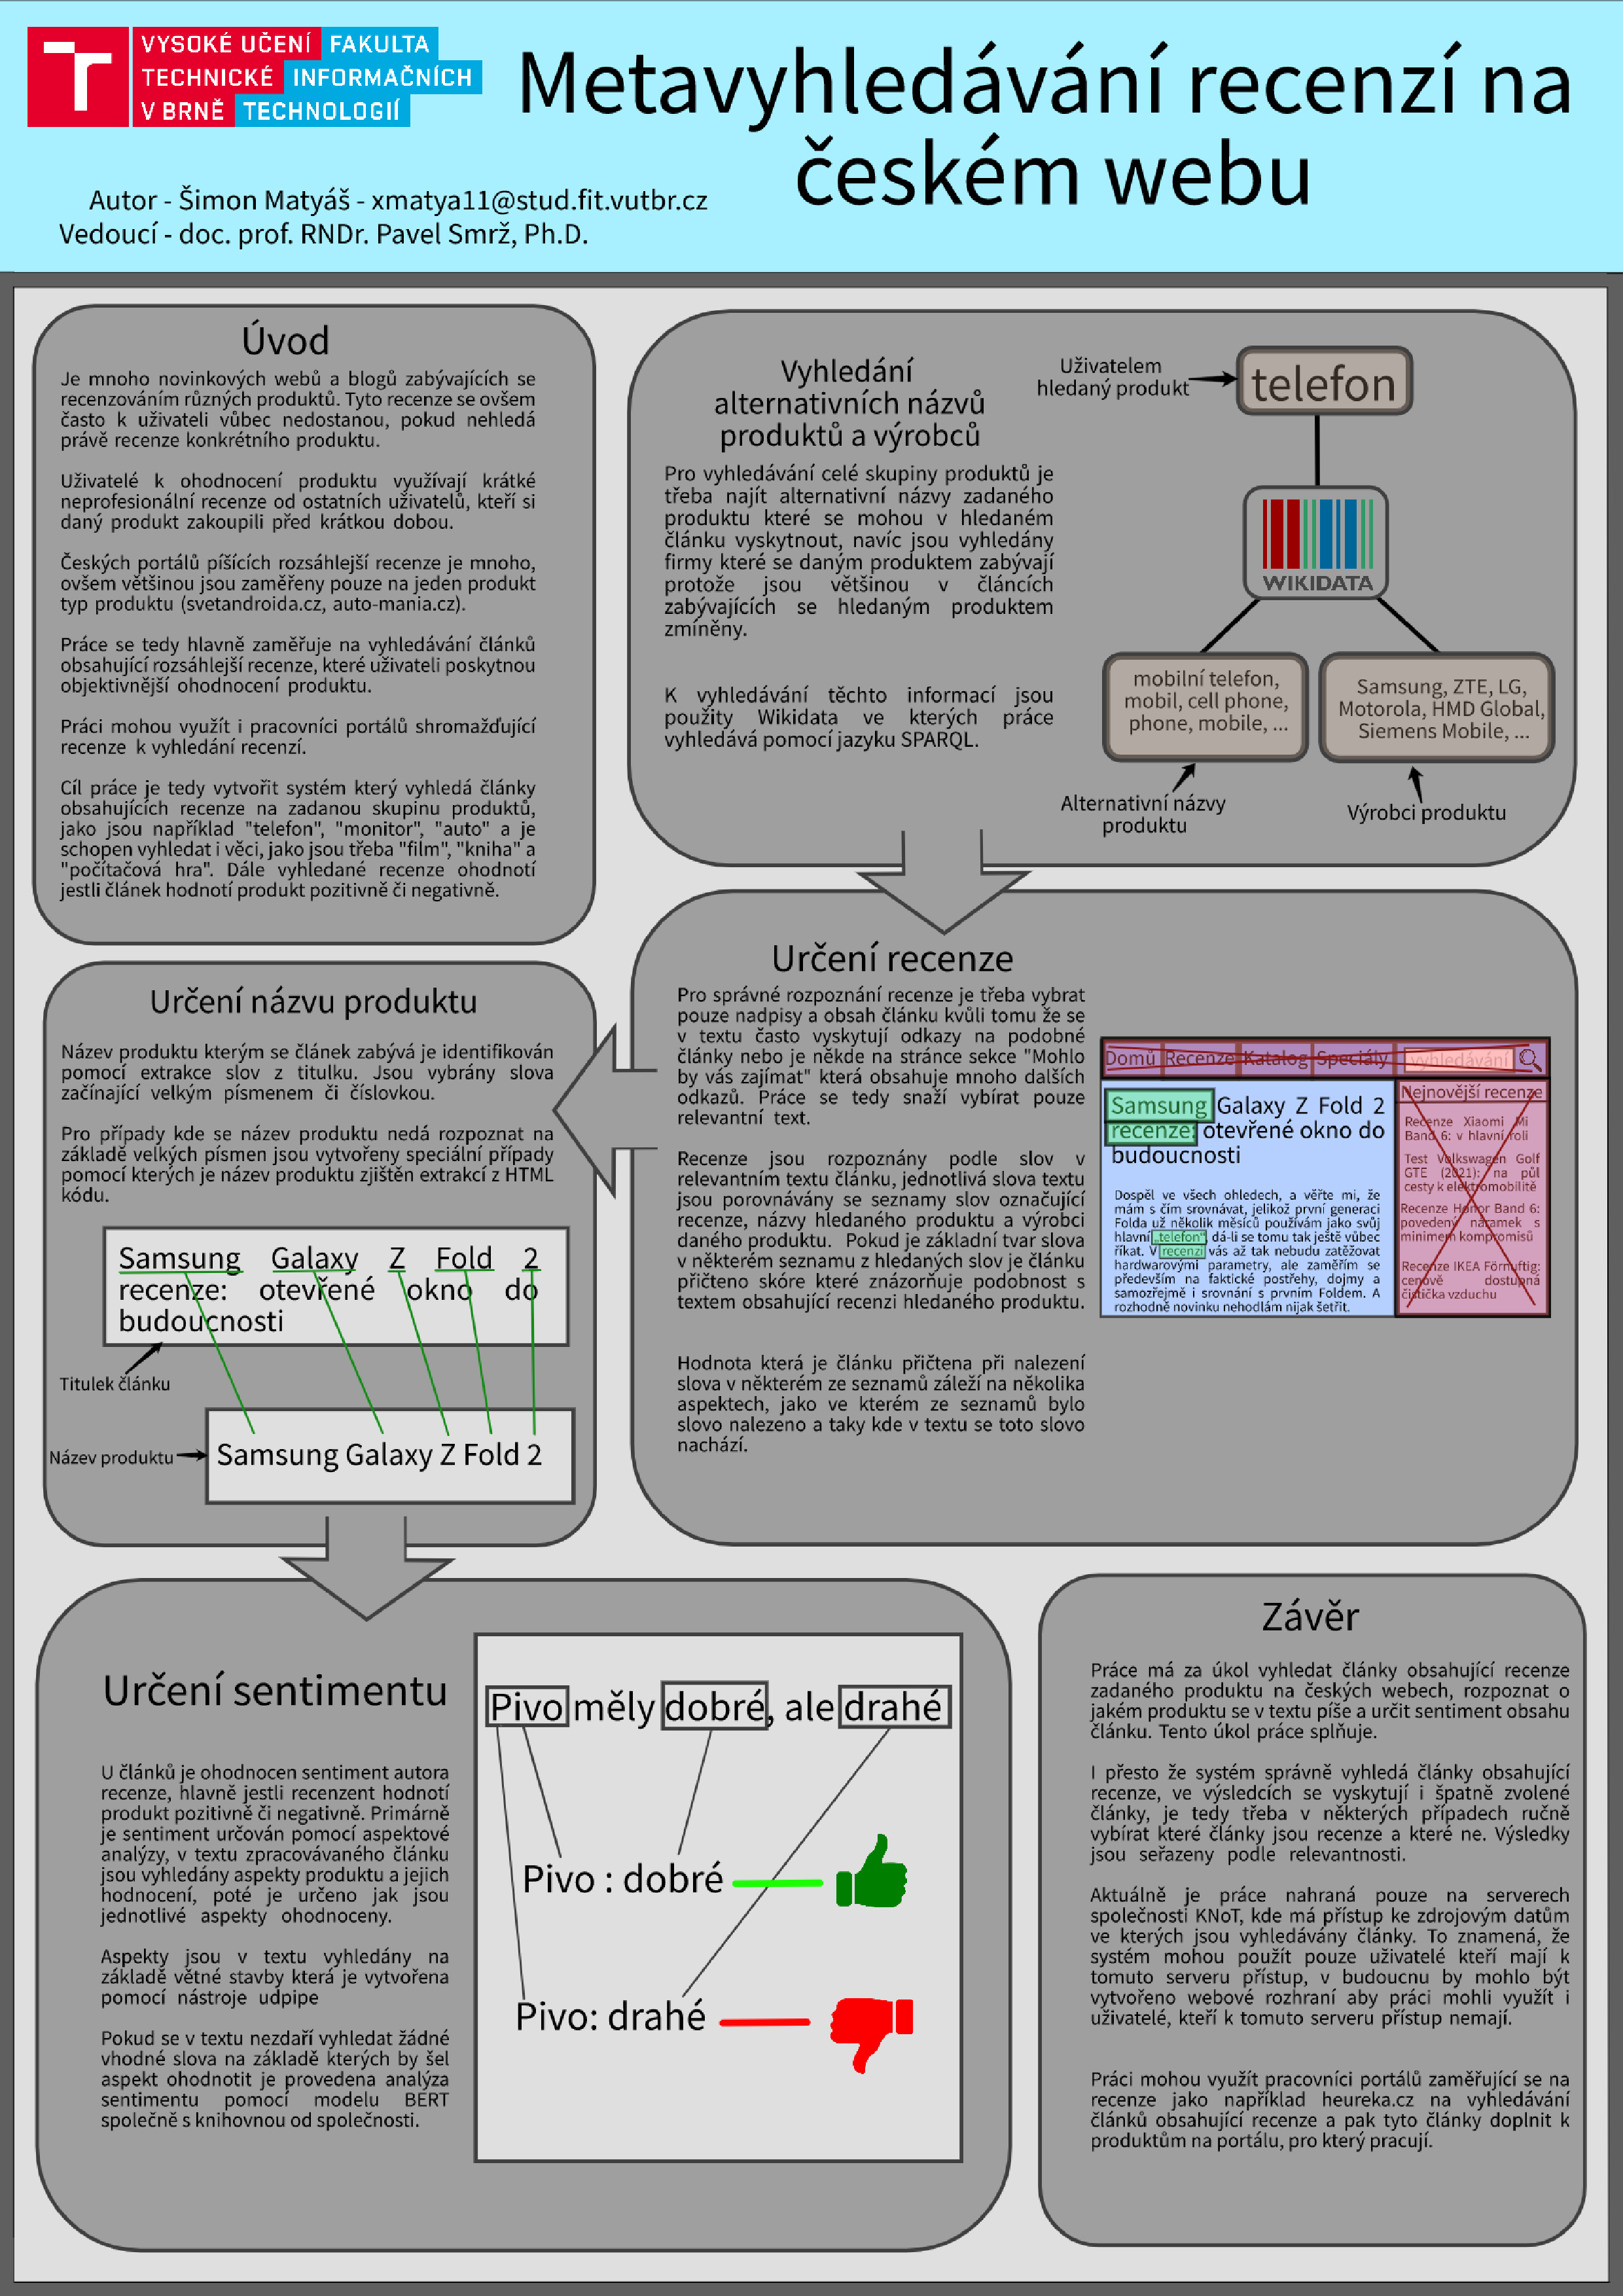
\includegraphics[scale=0.28]{obrazky-figures/plakat.pdf}
\end{center}
  \fi
  
  % Kompilace po částech (viz výše, nutno odkomentovat)
  % Compilation piecewise (see above, it is necessary to uncomment it)
  %\subfile{xmatya11-Metavyhledavani-recenzi-30-prilohy-appendices}
  
\end{document}
